\section{Terminology}
Queueing theory studies systems and processes in terms of three key concepts:
\begin{itemize}[noitemsep]
\item \textbf{customers} are the units of work that the system serves -- a customer can be a real person, or it can be whatever the system is supposed to process and complete: a web request, a database query, a part to be milled by a machine, etc.;
\item \textbf{servers} are the objects that do the processing work -- a server might be the cashier at the grocery store, a web server, a database server, a milling machine, etc., and 
\item \textbf{queues} are where the units of work wait if the server is busy and can not start the work as they arrive -- a queue may be a physical line, or reside in memory, etc. 
\end{itemize}
To begin understanding and describing queues, we must first have know and understand some useful probability distributions, as well as input and output processes.
\subsection{Exponential and Poisson Probability Distributions}
The \textbf{Poisson} and \textbf{exponential} distributions play a prominent role in queuing theory. The Poisson distribution counts the number of discrete events occurring in a fixed time period; it is closely connected to the exponential distribution, which (among other applications) measures the time between arrivals of the events. The Poisson distribution is a discrete distribution; the random variable can only take non-negative integer values. The exponential distribution can take any (nonnegative) real value.
\newl Consider the problem of determining the probability of $n$ arrivals being observed during a time interval of length $t$, where the following assumptions are made:
\begin{itemize}[noitemsep]
\item the probability that an arrival is observed during a small time interval (say of length $\nu$) is proportional to the length of interval; let the proportionality constant be $\lambda$, so that the probability is $\lambda\nu$;
\item the probability of two or more arrivals in a small interval is zero, and 
\item the number of arrivals in any time interval is independent of the number in non-overlapping time interval (for example, the number of arrivals occurring between times 5 and 25 does not provide information about the number of arrivals occurring between times 30 and 50).
\end{itemize}
\begin{figure}[!t]
\centering
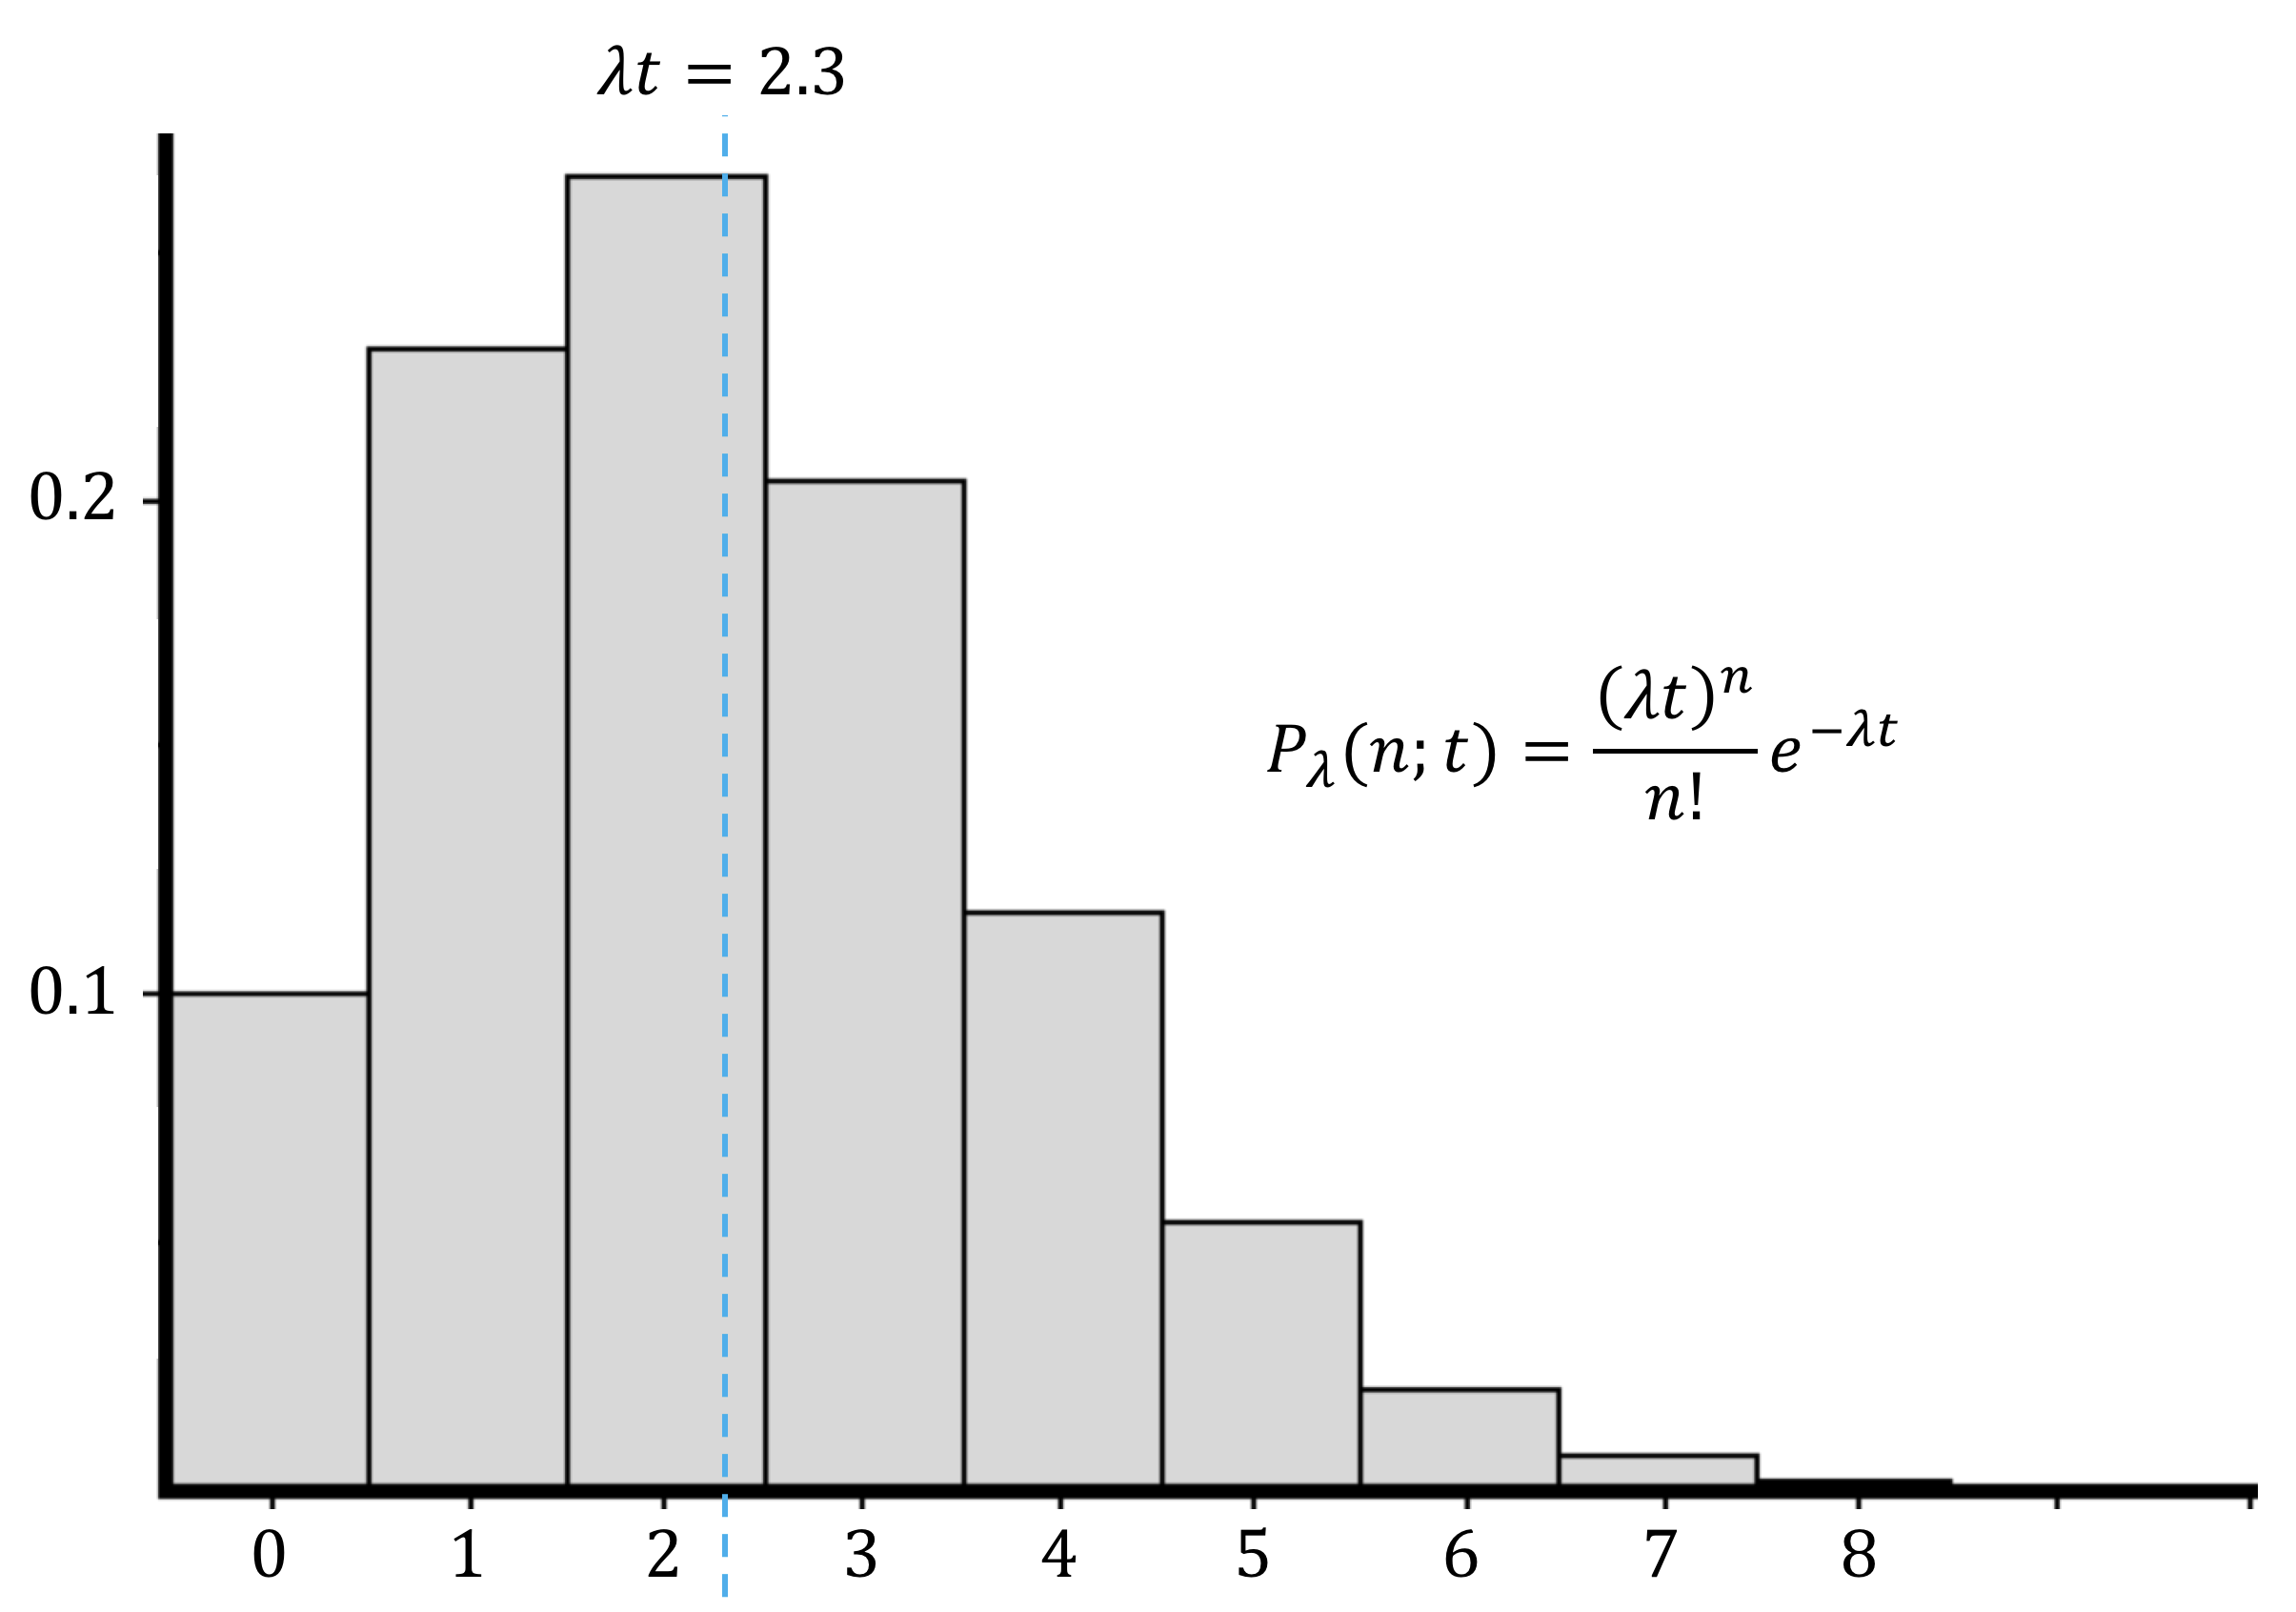
\includegraphics[height=0.25\textheight]{Images/poisson.png}
\centering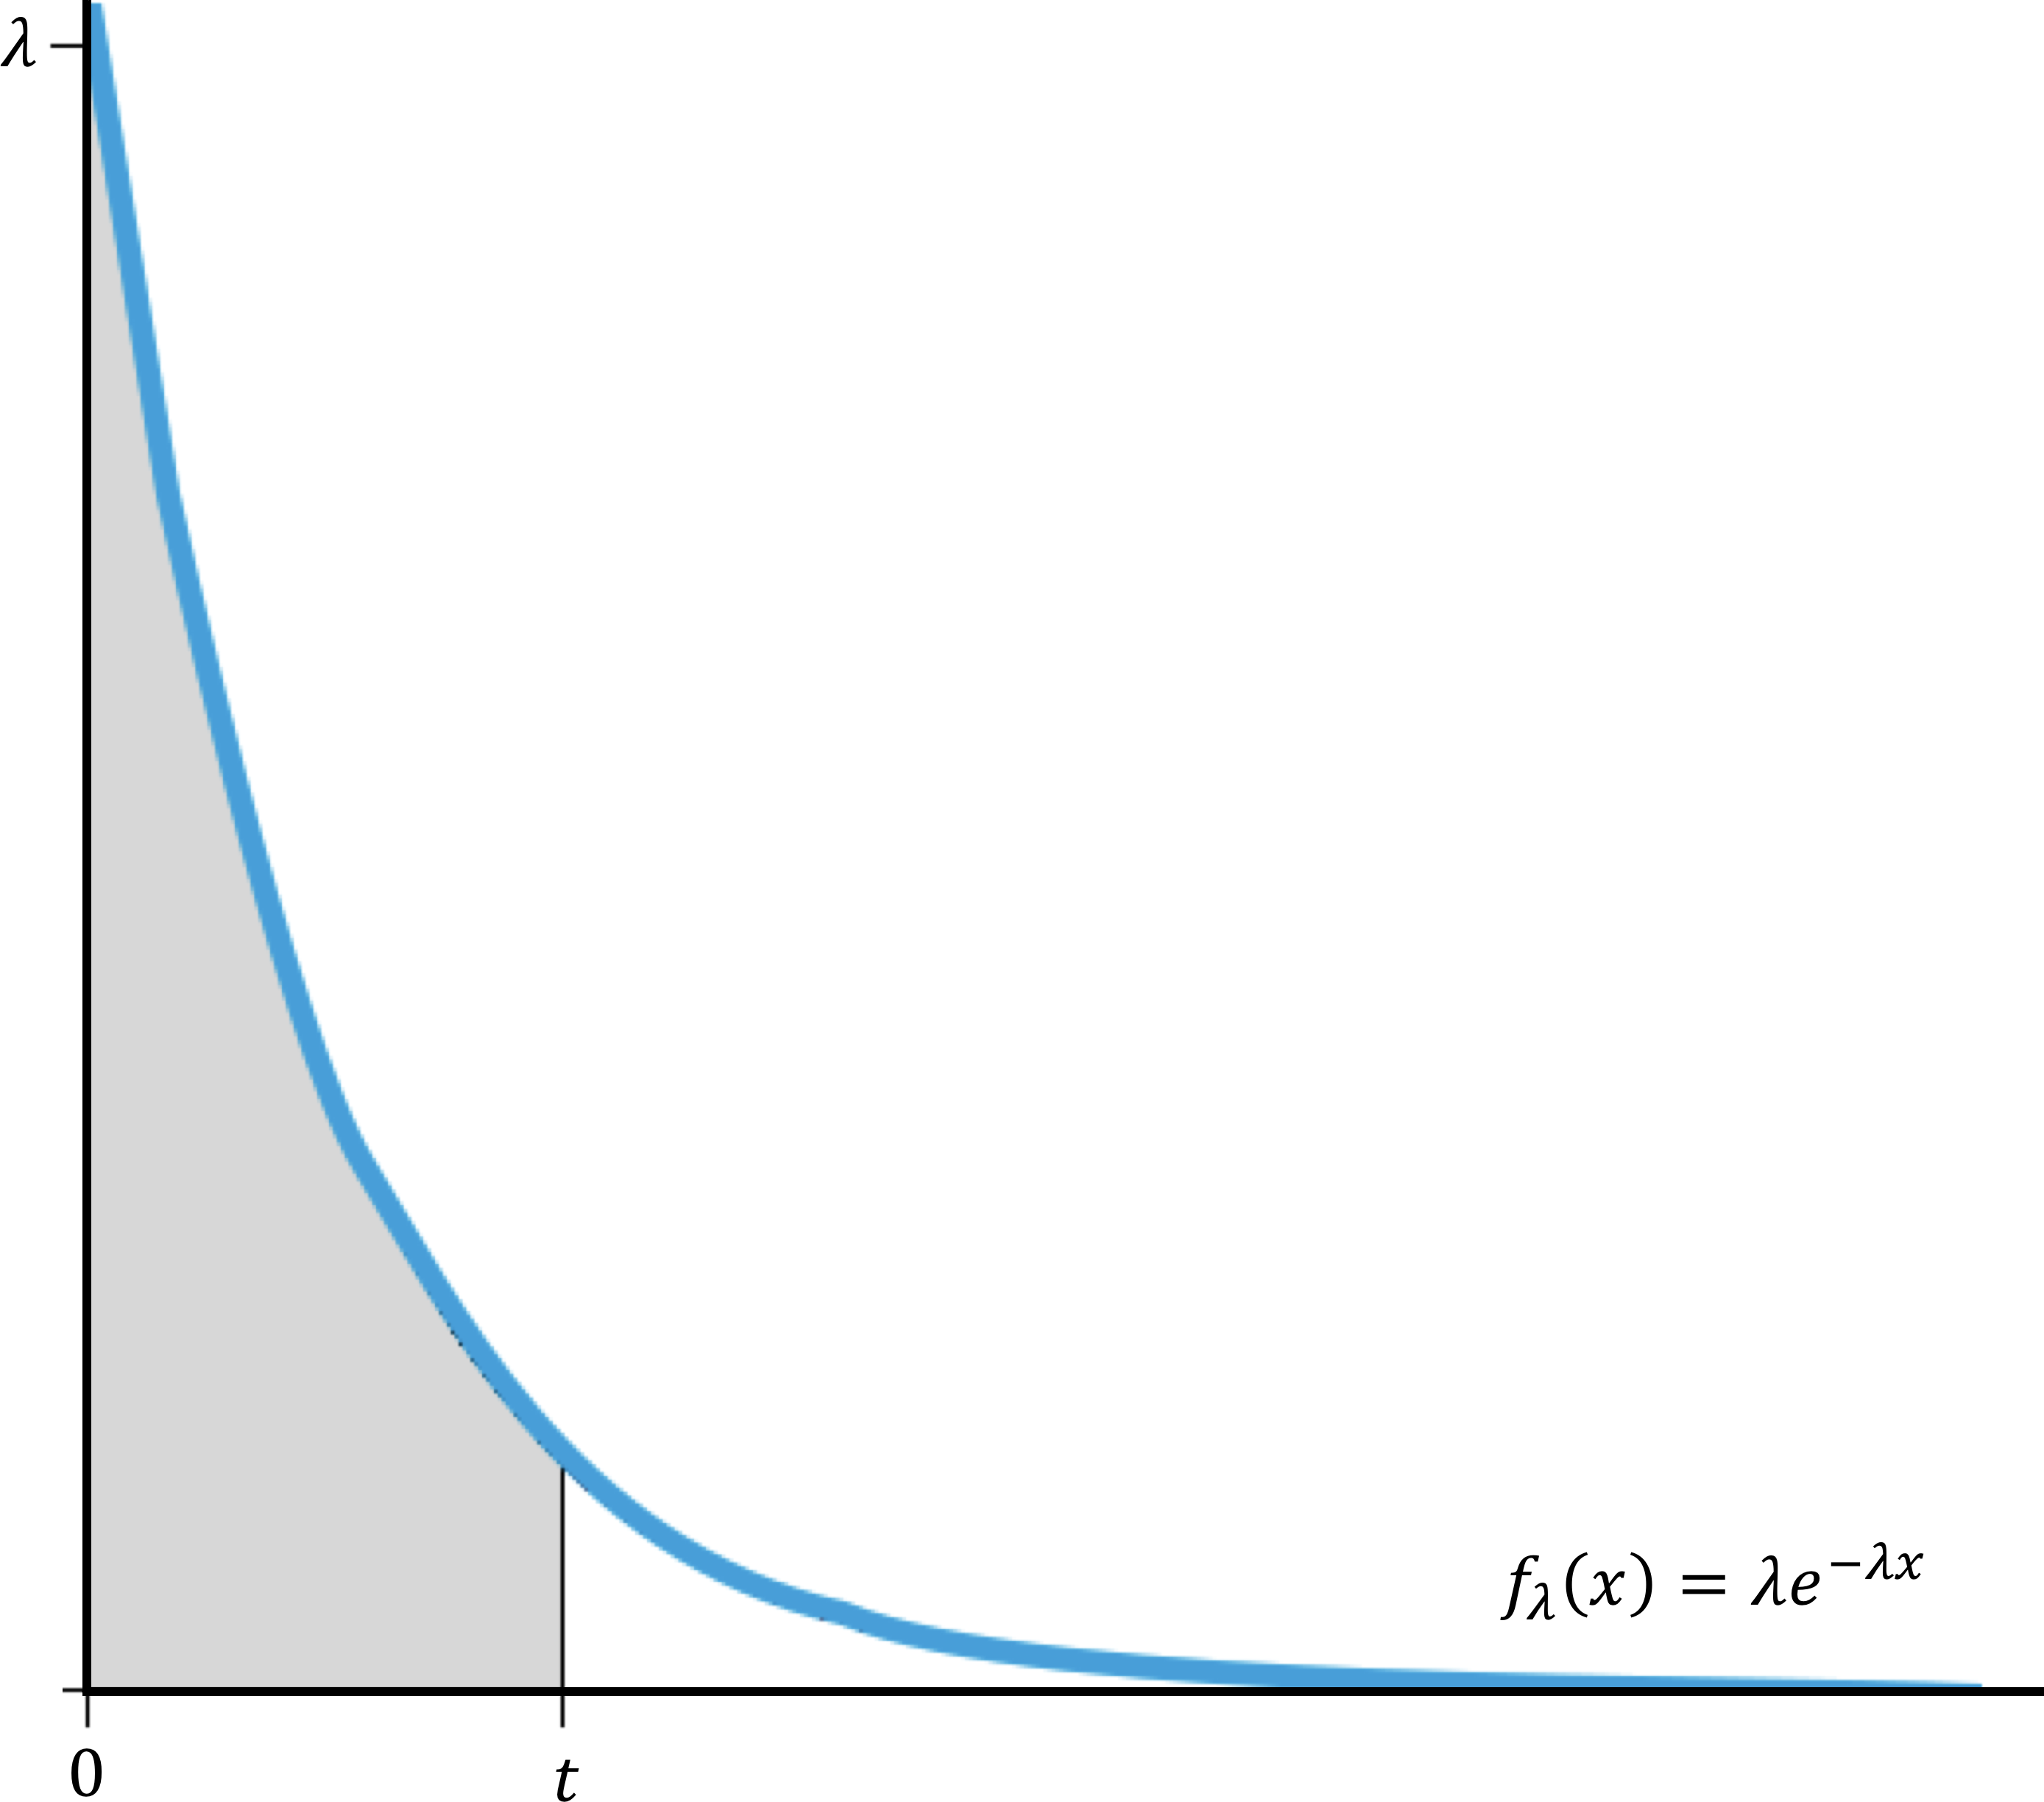
\includegraphics[height=0.25\textheight]{Images/exp.png}
\caption{\small Poisson (with $\lambda t=2.3$) and exponential distributions (with parameter $\lambda$). The shaded area (on the right) represents the probability that a customer will wait up to the length of the time interval $t$.}\label{fig:dist1}\hrule
\end{figure}
Now, let $P(n;t)$ be the probability of observing $n$ arrivals in a time interval of length $t$.
Then, for some $\lambda>0$, 
$$ P_{\lambda}(n; t) = \frac{(\lambda t)^n}{n!} e^{-\lambda t}, \ n=0,1,2,\cdots$$
is the p.m.f. of the \textbf{Poisson distribution} for the discrete random variable $n$ -- the number of arrivals -- for a given length of time interval $t$ (see Figure~\ref{fig:dist1}). In a queueing system, such arrivals are referred to as \textbf{Poisson arrivals}. \par The time between successive arrivals is called the \textbf{inter-arrival time}. If the number of arrivals in a given time interval follows a Poisson distribution with parameter $\lambda t$, the inter-arrival times follow an exponential distribution with p.d.f. 
$$ f_{\lambda}(t) = \lambda e^{-\lambda t}, \ \textrm{for }t>0,$$ and the probability $P(W\leq t)$ that a customer's waiting time $W$ is smaller than the length of the time interval $t$ is  
$$P(W\leq t) = 1 - e^{-\lambda t}\quad \textrm{(see Figure~\ref{fig:dist1})}.$$
In general, if the arrival rate is \textbf{stationary}, if \textbf{bulk} arrivals (two or more simultaneous arrivals) cannot occur, and if past arrivals do not affect future arrivals, then inter-arrival times follow an exponential distribution with parameter $\lambda$, and the number of arrivals in any interval of length $t$ is Poisson with parameter $\lambda t$. \newl One of the most attractive features of using the exponential distribution to model inter-arrival times is that it is \textbf{memoryless} --  if a random variable $X$ follows an exponential distribution, then for all non-negative values of $t$ and $h$,
\begin{equation}
P(X \geq t + h|X \geq t) = P(X \geq h). 
\label{eq:1}
\end{equation}
No other density function satisfies $(\ref{eq:1})$ \cite{QS_R}. The memoryless property of the exponential distribution is important because it implies that the probability distribution of the time until the next arrival is independent of the time since the last arrival -- imagine if that was the case when waiting for public transportation! \par For instance, if we know that at least $t$ time units have elapsed since the last arrival, then the distribution of time $h$ until the next arrival is independent of $t$. If $h=4$, say, then $(\ref{eq:1})$ yields 
$$ P(X>9|X>5)= P(X>7|X>3) = P(X>4|X>0) = e^{-4 \lambda}.$$

\subsection{Erlang Distribution}
The exponential distribution is not always an appropriate model of inter-arrival times (perhaps the process should not be memoryless, say). A common alternative is to use the \textbf{Erlang} distribution $\mathcal{E}(R,k)$, a continuous random variable with \textbf{rate} and \textbf{shape} parameter $R>0$ and $k\in \mathbb{Z}^+$, respectively, whose p.d.f. is  
$$ f_{R,k}(t) = \frac{R (Rt)^{k-1} e^{-Rt}}{(k-1)!},\ t\geq 0.$$
When $k=1$, the Erlang distribution reduces to an exponential distribution with parameter $R$. It can be shown that if $X\sim \mathcal{E}(k\lambda,k)$, then  $X\sim X_{1}+X_{2}+\cdots+X_{k},$ where each $X_{i}$ is an independent exponential random variable with parameter $k \lambda$. \newl When we model the inter-arrival process as an Erlang $\mathcal{E}(k\lambda,k)$ distribution, we are really saying that it is equivalent to customers going through $k$ \textbf{phases} (each of which is memoryless) before being served. For this reason, the shape parameter is often referred to as the number of phases of the Erlang distribution \cite{QS_N}.
\subsection{Input/Arrival Process}
The input process is usually called the \textbf{arrival process}. Arrivals are called \textbf{customers}. In the models that we discuss, we assume that arrivals cannot be simultaneous (this might be unrealistic when modeling a restaurant, say). If simultaneous arrivals can occur, we say that \textbf{bulk arrivals are allowed}. 
\par Usually, we assume that the arrival process is \textbf{unaffected by the number of customers} in the system. In the context of a bank, this would imply that whether there are 500 or 5 people at the bank, the process governing arrivals remains unchanged.  
\newl There are two common situations in which the arrival process may depend on the number of customers present. The first occurs when arrivals are drawn from a small population -- the so-called \textbf{finite source models} -- if all members of the populations are already in the system, there cannot be another arrival!\par Another such situation arises when the rate at which customers arrive at the facility decreases when the facility becomes too crowded. For example, when customers see that a restaurant's parking lot is full, they might very well decide to go to another restaurant or forego eating out altogether. If a customer arrives but fails to enter the system, we say that the customer has \textbf{balked}.
\subsection{Output/Service Process}
To describe the output process (often called the \textbf{service process}) of a queuing system, we usually specify a probability distribution -- the \textbf{service time distribution} -- which governs the customers' service time. \newpage\noindent In most cases, we assume that the service time distribution is independent of the number of customers present in the system. This implies, for example, that the server does not work faster when more customers are present. \newl We can distinguish two types of servers: \textbf{in parallel} and \textbf{in series}. Servers are in parallel if they all provide the same type of service and a customer only needs to pass through one of them to complete their service. For example, the tellers in a bank are usually arranged in parallel; typically, customers only need to be serviced by one teller, and any teller can perform the desired service. Servers are in series if a customer must pass through several servers before their service is complete. An assembly line is an example of such a queuing system.
\newl 
Input and output processes occur in a variety of situations:
\begin{itemize}[noitemsep]
\item \textbf{situation:} purchasing Blue Jays tickets at the Rogers Centre\\ \textit{input:} baseball fans arrive at the ticket office\\ \textit{output:} tellers serve the baseball fans;
\item \textbf{situation:} pizza parlour \\ \textit{input:} requests for pizza delivery are received; \textit{output}: pizza parlour prepares and bakes pizzas, and sends them to be delivered; 
\item \textbf{situation:} government service centre\\ \textit{input}: citizen/residents enter the service centre \\ \textit{output:} receptionist assigns them to a specific queue based on their needs\\
\textcolor{white}{.}\qquad \textit{input:} citizen/residents enter a specific queue based on their needs \\ \textcolor{white}{.}\qquad \textit{output:} public servant addresses their needs;
\item \textbf{situation:} hospital blood bank\\ \textit{input:} pints of blood arrive\\ \textit{output:} patients use up pints of blood;
\item \textbf{situation:} garage\\ \textit{input:} cars break-down and are sent to the garage for repairs\\ \textit{output:} cars are repaired by mechanics and sent back on the streets.
\end{itemize}
The computations are fairly easy to execute, as the following examples demonstrate.
\begin{itemize}
\item On average, 4.6 customers enter a coffee shop each hour. If the arrivals follow a Poisson process, the probability that at most two customers will enter in a 30 minute period is \begin{align*}P_{\lambda=4.6}(n\leq 2;t=0.5)&=P_{4.6}(0,0.5)+P_{4.6}(1,0.5)+P_{4.6}(2,0.5) \\ &=e^{-4.6\cdot 0.5}\left[\frac{(4.6\cdot 0.5)^0}{0!}+\frac{(4.6\cdot 0.5)^1}{1!}+\frac{(4.6\cdot 0.5)^2}{2!}\right] \\ &\approx 0.5960; \end{align*} the corresponding Poisson distribution is shown in Figure~\ref{fig:dist1}. 
\item In a fast food restaurant, a cashier serves on average 9 customers in a one-hour time period. If the service time follows an exponential distribution, $89.5\%$ and $2.4\%$ of customers will be served in 15 minutes or less and after 25 minutes, respectively. Indeed, $$P(W\leq 15/60)=1-e^{-9 \cdot 15/60} \approx 0.8946\quad\text{and}\quad P(W>25/60)=e^{-9\cdot 25/60}\approx 0.0235.$$	
\end{itemize}

\subsection{Queue Discipline}
To describe a queuing system completely, we must also describe the \textbf{queue discipline} and the manner in which customers \textbf{join lines}. The queue discipline describes the method used to determine the order in which customers are served: 
\begin{itemize}[noitemsep]
\item the most common queue discipline is the \textbf{first come, first served} (FCFS) discipline, in which customers are served in the order of their arrival, as one would expect to see in an Ottawa coffee shop;
\item under the \textbf{last come, first served} (LCFS) discipline, the most recent arrivals are the first to enter service; for example, if we consider exiting from an elevator to be the service, then a crowded elevator illustrates such a discipline;
\item sometimes the order in which customers arrive has no effect on the order in which they are served; this would be the case if the next customer to enter service is randomly chosen from those customers waiting for service, a situation referred to as \textbf{service in random order} (SIRO) discipline; when callers to an inter-city bus company are put on hold, the luck of the draw often determines which caller will next be serviced by an operator, 
\item finally, \textbf{priority} discipline classifies each arrival into one of several categories, each of which is assigned a priority level (a \textbf{triage} process); within each priority level, customers enter the queue on a FCFS basis; such a discipline is often used in emergency rooms to determine the order in which customers receive treatment, and in copying and computer time-sharing facilities, where priority is usually given to jobs with shorter processing times.
\end{itemize}

\subsection{Method Used by Arrivals to Join Queue}
Another important factor for the behaviour of the queuing system is the \textbf{method} used by customers to determine which line to join. For example, in some banks, customers must join a single line, but in other banks, customers may choose the line they want to join. \par  When there are several lines, customers often join the shortest line. Unfortunately, in many situations (such as at a supermarket), it is difficult to define the shortest line. If there are several lines at a queuing facility, it is important to know whether or not customers are allowed to \textbf{switch}, or jockey, between lines. In most queuing systems with multiple lines, jockeying
is permitted, but jockeying at a custom inspection booth would not be recommended, for instance. 

%%%%%________________Section3_________________________%%%%

\section{Queueing Theory Framework}
There is a standard notation that is used to describe large families of queueing systems.
\subsection{Kendall-Lee Notation}
Queuing systems can be described by six characteristics \cite{QS_K}: $$x_1/x_2/x_3/x_4/x_5/x_6.$$
The first characteristic $x_1$ specifies the nature of the \textbf{arrival process}. The following standard abbreviations are used:
\newl \begin{tabular}{p{0.25cm}p{0.25cm}p{15cm}}
$M$ &$=$& inter-arrival times are independent, identically distributed (iid) exponentials\\
$D$ &$=$& inter-arrival times are iid and deterministic\\
$E_{k}$ &$=$& inter-arrival times are iid Erlangs with shape parameter $k$\\
$G$ &$=$& inter-arrival times are iid and governed by some general distribution.
\end{tabular}
\newpage\noindent
The second characteristic $x_2$ specifies the nature of the \textbf{service times}:
\newline \newline
\begin{tabular}{p{0.25cm}p{0,25cm}p{12cm}}
$M$ &$=$& service times are iid and exponential\\
$D$ &$=$&  service times are iid and deterministic.\\
$E_{k}$ &$=$& service times are iid Erlang with shape parameter $k$\\
$G$ &$=$& service times are iid and follow some general distribution.
\end{tabular}
\newl
The third characteristic $x_3$ is the \textbf{number of parallel servers}. The fourth characteristic $x_4$ describes
the \textbf{queue discipline}:
\newl
\begin{tabular}{ccc}
FCFS &$=$& first come, first served\\
LCFS &$=$& last come, first served\\
SIRO &$=$& service in random order\\
GD &$=$& general queue discipline.
\end{tabular}
\newl
The fifth characteristic $x_5$ specifies the \textbf{maximum allowable number of customers in the system} (including customers who are waiting and customers who are in service). The sixth characteristic $x_6$ gives the \textbf{size of the population} from which customers are drawn. Unless
the number of potential customers is of the same order of magnitude as the number of servers, the population size is considered to be infinite. \newl In many important models $x_4/x_5/x_6$ is $\textrm{GD}/\infty/\infty$; when this is the case, these characteristics are often omitted.  For example, $M/M/3/\textrm{FCFS}/20/\infty$ could represent a bank with 3 tellers, exponential arrival times, exponential service times, a ``first come, first served'' queue discipline, a total capacity of 20 customers, and an infinite population pool from which to draw. The situation is partly illustrated in Figure~\ref{fig:1}.
\begin{figure}[!t]
	\centering
		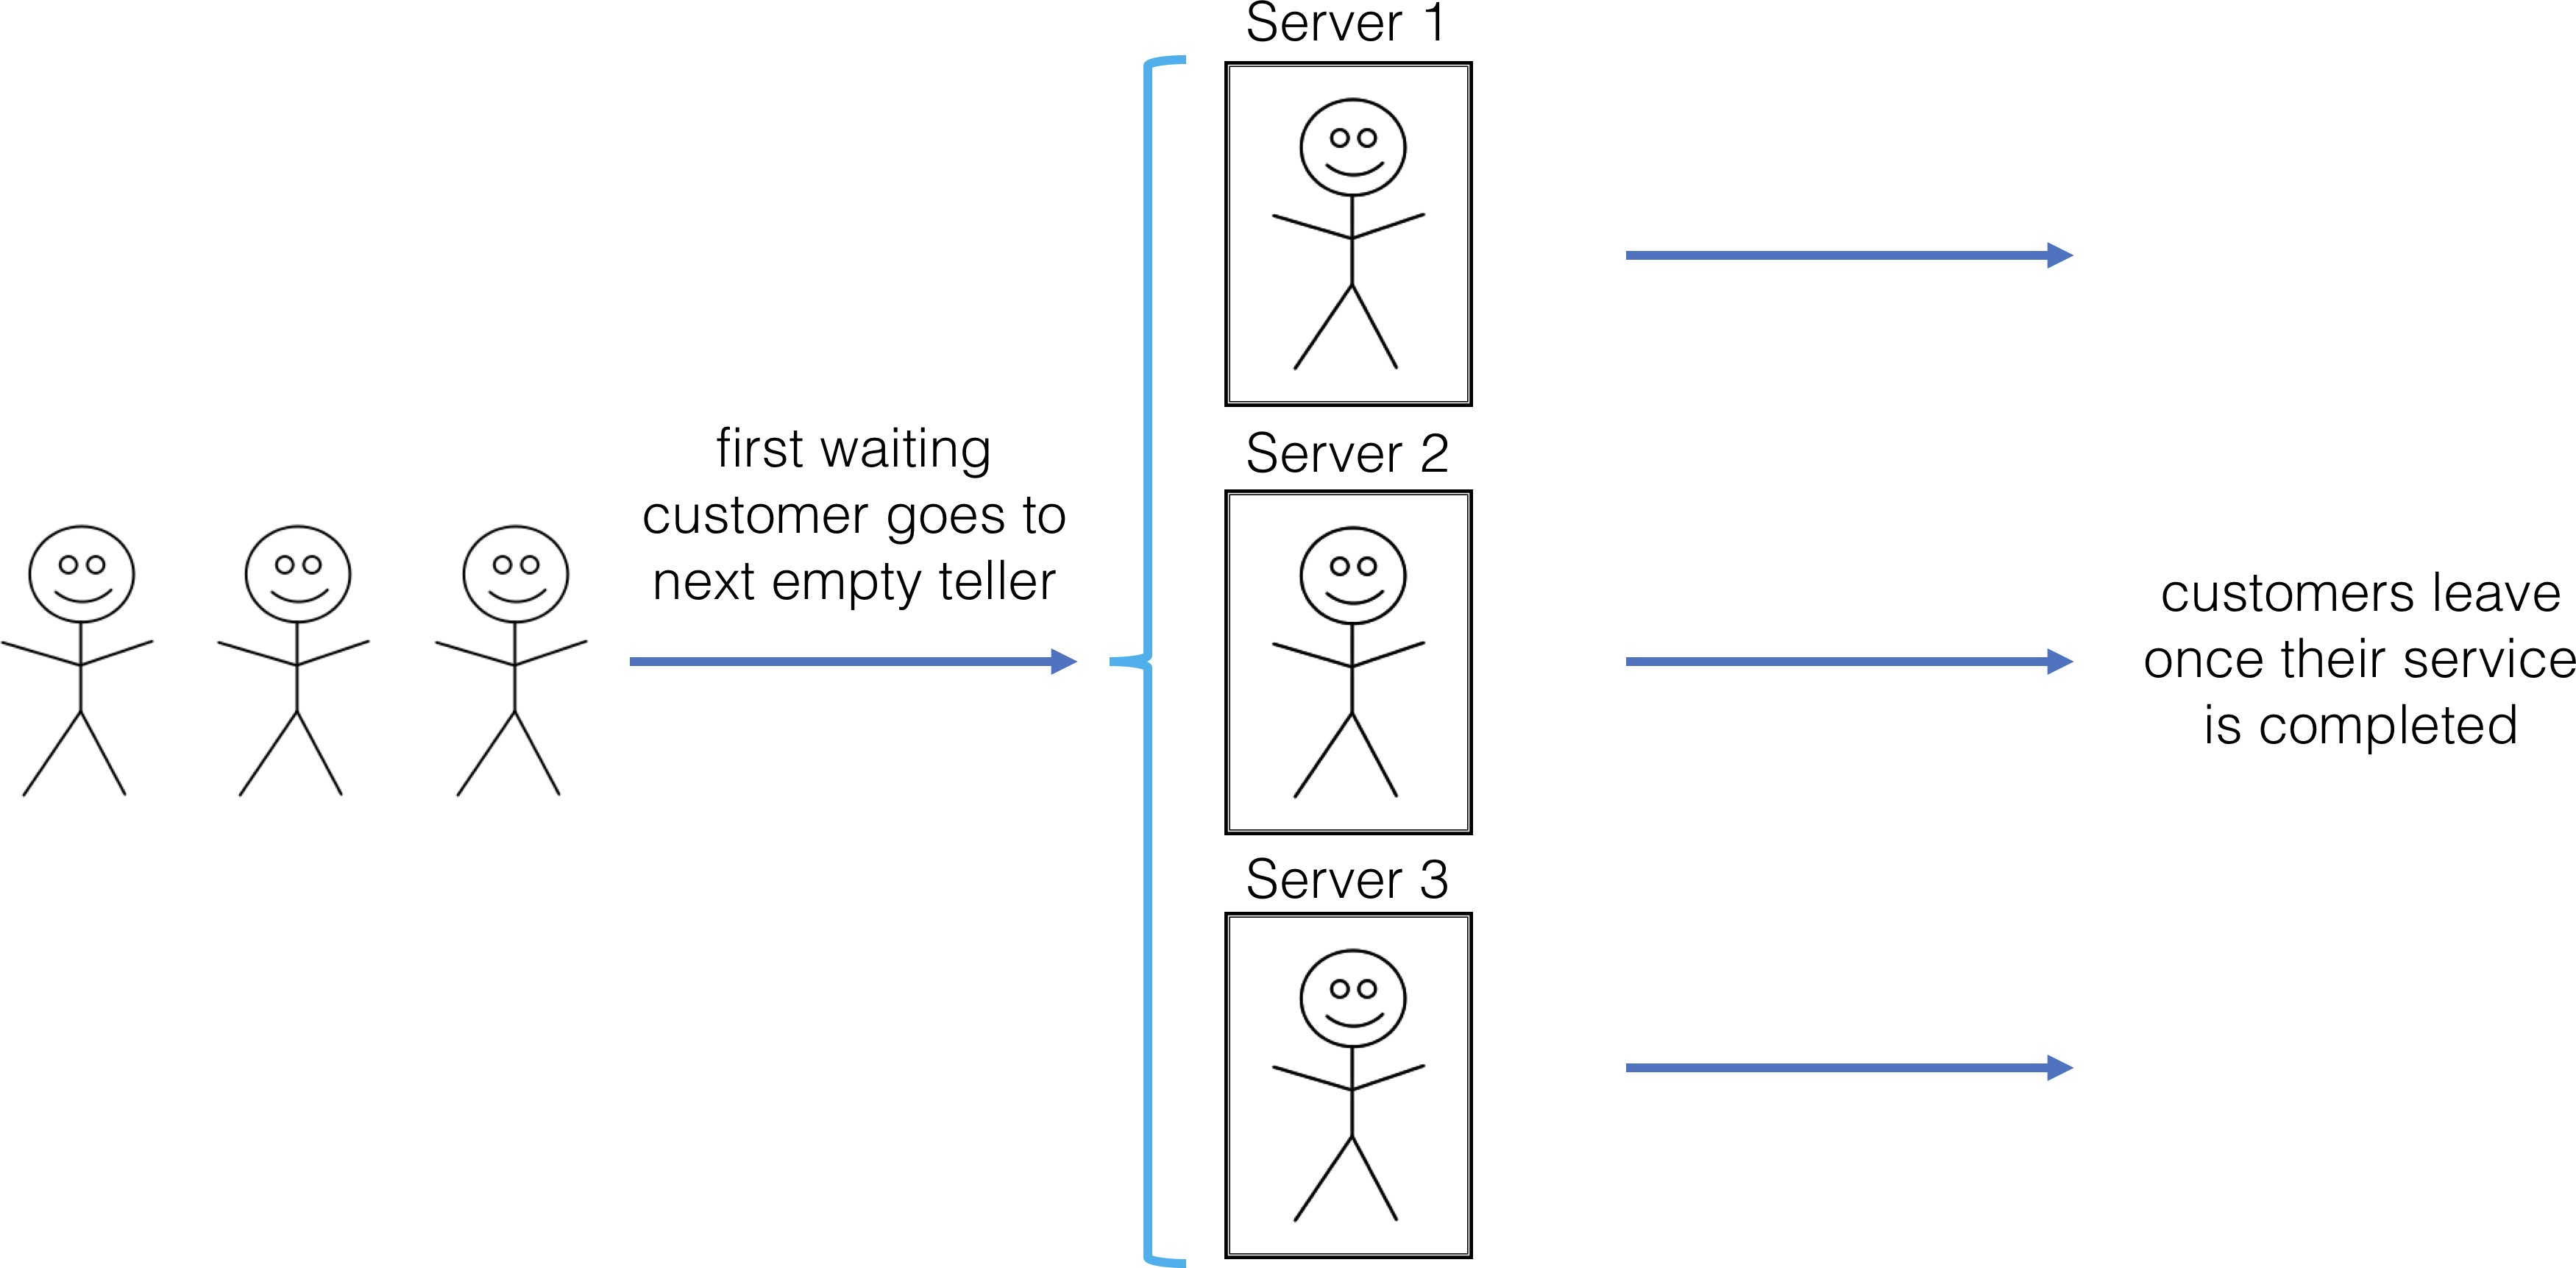
\includegraphics[width=\textwidth]{Images/fig1Queue.png}
	\caption[\small Single line at bank with three tellers]{\small Single line at bank with three tellers -- $M/M/3/\textrm{FCFS}/20/\infty$.}
	\label{fig:1}\hrule
\end{figure}
\vfill

\subsection{Birth-Death Processes}
\begin{figure}[!t]
	\centering
		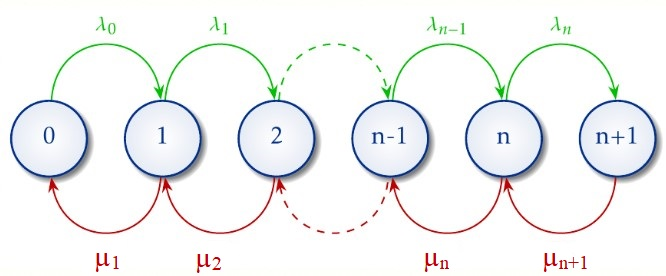
\includegraphics[width=0.99\textwidth]{Images/fig2Queue.jpg}
	\caption[\small Birth-death process]{\small Birth-death Process; queueing states indexed by integers; birth rates and death rates indicated by $\lambda_n$ and $\mu_m$, respectively.}
	\label{fig:2}\hrule
\end{figure}
\afterpage{\FloatBarrier}
\noindent The \textbf{state of a queueing system} at time $t$ is defined to be the number of customers in the queuing system, either waiting in line or in service, at time $t$. At $t = 0$, the state of the system is  the initial number of customers in the system. This state is noteworthy because it clearly affects the state at future $t$. \par Knowing this, we define $P_{ij} (t)$ as the probability that the state at time $t$ is $j$, given that the state at $t = 0$ was $i$. For large $t$, $P_{ij} (t)$ becomes independent of $i$ and approaches a limit $\pi_{j}$. This limit is known as the \textbf{steady-state} of state $j$.\par It is generally incredibly difficult to determine the steps of arrivals and services that lead to a steady-state $\pi_j$. Likewise, starting from a small $t$, it is difficult to determine exactly when a system will reach
its steady state $\pi_j$, if such a state even exists. \par For simplicity's sake, when a queuing system is studied, we begin by assuming that the steady-state has already been reached.\newl  
A \textbf{birth-death process} is a Markov process in which states are indexed by non-negative integers, and transitions are only permitted between ``neighbouring'' states. After a ``birth'', the state increases from $n$ to $n+1$; after a ``death'', the state decreases from $m$ to $m-1$. Typically, we denote the set of birth rates and death rates by $\lambda_n$ and $\mu_m$, respectively (see Figure~\ref{fig:2}). \textbf{Pure birth} processes are those for which $\mu_m=0$ for all $m$; \textbf{pure death} processes those for which $\lambda_n=0$ for all $n$. The  \textbf{steady-state solution} of a birth-death process, i.e. the probability $p_n$ of being in state $n$ \textit{can} actually be computed: 
\begin{align} p_{n} &= p_{0}\frac{\lambda_{0} \lambda_{1} \cdots \lambda_{n-1}}{\mu_{1} \mu_{2} \cdots \mu_{n}},\quad  \text{for    } n=1,2,\cdots,\label{eq:ssbr}
\end{align}
where $p_{0}$ is  the probability of being in state 0. It can further be shown  \cite{QS_K1} that:
$$ p_{0} = \frac{1}{1+ \sum^{\infty}_{n=1} \prod^{n-1}_{j=0} \frac{\lambda_{j}}{\mu_{j+1}}}.$$ 

\subsection{Little's Queuing Formula}
It is often the case that a client is interested in the amount of time that a typical customer spends in the queuing system. Let $W$ be the \textbf{expected waiting time} spent in the queuing system, including time in line plus time in service, and $W_{q}$ be the \textbf{expected time a customer spends waiting in line}. Both $W$ and $W_{q}$ are computed under the assumption that the steady state has been reached. By using a powerful result known as \textbf{Little's queuing formula}, $W$ and $W_{q}$ are easily related to the number of customers in the queue and those waiting in line. \newl  For any queuing system (or any subset of a queuing system), consider the following quantities:
\begin{itemize}[noitemsep]
\item $\lambda = $  average number of arrivals entering the system per unit time; 
\item $L =$  average number of customers present in the queuing system;
\item $L_{q} = $  average number of customers waiting in line;
\item $L_{s} = $  average number of customers in service;
\item $W = $  average time a customer spends in the system;
\item $W_{q} = $  average time a customer spends in line, and
\item $W_{s} = $  average time a customer spends in service.
\end{itemize}
But customers in the system can only either be found in the queue or in service, so that $L = L_{q} + L_{s}$ as well $W = W_{q} + W_{s}$.  In these definitions, all averages are steady-state averages. For most queuing systems in which a steady-state exists, Little's queuing formula can be summarized as 
\begin{align*}
L &=  \lambda W, \quad L_{q} = \lambda W_{q}, \quad\mbox{and}
\quad L_{s}= \lambda W_{s}.
\end{align*}
For instance, if 46 customers enter a restaurant each hour it is opened (on average), and if they spend 10 minutes waiting to be served (on average), then we should expect $46\cdot 1/6 \approx 7.7$ customers in the queue at all time (on average).   

%%%%%%%%%%%%%%%%%%%%%% section 4%%%%%%%%%%%%%%%%%%%%%
\section{The $M/M/1$ Queuing System}
\subsection{Basics} An $M/M/1/\textrm{GD}/\infty/\infty$ system has exponential inter-arrival times, exponential service times, and a single server. It is the simplest non-trivial queueing system to analyse as it can be modeled as a birth-death process with
\begin{align*}
\lambda_{j} &= \lambda, \ j=0,1,2,\ldots \\ 
\mu_{0} &= 0 \\
\mu_{j} &= \mu,\  j=1,2,3,\ldots 
\end{align*}
Substituting these rates in (\ref{eq:ssbr}) yields 
$$\pi_{j} = \frac{\lambda^{j} \pi_{0}}{\mu^{j}}=\rho^j \pi_0,$$ where $\rho = \lambda/\mu$ is the \textbf{traffic intensity} of the system. Since the system has to be in exactly one of the states at any given moment, the sum of all probabilities is 1, or $$ \pi_{0}+\pi_1 + \pi_2+\cdots = \pi_0(1+\rho+\rho^{2}+\cdots ) = 1.$$
If $0 \leq \rho < 1$ the infinite series converges to $\frac{1}{1-\rho}$ from which we derive $$\pi_{0}\cdot \frac{1}{1-\rho} = 1 \implies \pi_0 = 1-\rho \implies \pi_{j} = \rho^{j} \pi_0 = \rho^j (1-\rho)$$
as the \textbf{steady-state probability of state $j$}.  If $\rho \geq 1$, the infinite series diverges and no steady-state exists. Intuitively, this happens when $\lambda \geq \mu$ -- if the arrival rate is greater than the service rate, then the state of the system grows without bounds and the queue is never cleared.
\newl From this point on, we assume $\rho < 1$ to guarantee that the steady-state probabilities $\pi_{j}$  exist, from which we can determine several quantities of interest. Assuming
that the steady state has been reached, it can be shown that $L$, $L_{s}$, and $L_{q}$ are given respectively by:
\begin{align*}
L &= \frac{\lambda}{\mu - \lambda}\\
L_{s} &= \rho\\
 L_{q} &= \frac{\rho^{2}}{1-\rho}.
 \end{align*}
Using Little's queuing formula, we can also solve for $W$, $W_{s}$, and $W_{q}$ by dividing each of the corresponding $L$ values by $\lambda$.  Notice that, as expected, both $W$ and $W_{q}$ when $\rho\to 1$. On the other hand, $W_{q}\to 0$ and $W\to \frac{1}{\mu}$ (the \textbf{mean service time}) as $\rho\to 0$.
\newl 
(The following example is based on \cite{QS_W}) An average of 10 cars arrive at a single-server drive-in teller every hour. If the average customer is served in 4 minutes, service time for each customer is 4 minutes, and both inter-arrival times and service times are exponential, then: \begin{itemize}[noitemsep]
	\item[(a)] What is the probability that the teller is idle? 
	\item[(b)] Excluding the car that is being served, what is the average number of cars waiting in line at the teller? 
	\item[(c)] What is the average amount of time a drive-in customer spends in the bank parking lot (including time in service)?
	\item[(d)] On average, how many customers per hour will be served by the teller?
\end{itemize}
By assumption, we are dealing with an $M/M/1/\textrm{GD}/\infty/\infty$ queuing system for which $\lambda = 10$ cars/hr and $\mu = 15$ cars/hr, and as such  $\rho = 10/15 = 2/3$.
\begin{itemize}[noitemsep]
	\item[(a)] The teller is idle one third of the time on average because $\pi_{0} = 1 - \rho = 1/3$.
	\item[(b)] There are $L_{q} = \rho^{2}/(1-\rho) = 4/3$ cars waiting in line for the teller. 
	\item[(c)] We know that $L = \lambda/(\mu - \lambda) = 10/(15-10) = 2$, and so $W = L/\lambda = 0.2 \textrm{ hr} = 12 \textrm{ min}$.
	\item[(d)] If the teller were always busy, it would serve an average of $\mu = 15$ customers per hour. From (a), we know that the teller is only busy two-thirds of the time, thus during each hour, the teller serves an average of $15 \cdot 2/3 = 10$ customers. This is reasonable since, in a steady-state, $10$ customers are arriving each hour and $10$ customers must leave the system every hour.
\end{itemize}
\newpage\noindent
(This next example is based on \cite{QS_E}) Suppose that all car owners fill up when their tanks are exactly half full.  At the present time, an average of $7.5$ customers arrive every hour at a single-pump gas station. It takes an average of $4$ minutes to fuel a car. Assume that inter-arrival times and service times are both exponential. \begin{itemize}[noitemsep]
	\item[(a)] What are the values of $L$ and $W$ in this scenario? 
	\item[(b)] Suppose that a gas shortage occurs and panic buying takes place. To model this phenomenon, assume that all car owners now purchase gas when their tanks are exactly three-quarters full. Since each car owner is now putting less gas into the tank during each visit to the station, we assume that the average service time has been reduced to $10/3$ minutes. How has panic buying affected the values of $L$ and $W$?
\end{itemize}
By assumption, we have again an $M/M/1/\textrm{GD}/\infty/\infty$ queuing system, this time with $\lambda = 7.5$ cars/hr and $\mu = 60/4 = 15$ cars/hr.  Thus, $\rho = 7.5/15 = 1/2$.
\begin{enumerate}[noitemsep]
	\item[(a)] By definition, $L = \lambda/(\mu - \lambda) = 7.5/(15-7.5) = 1$ and $W = 1/7.5 \approx 0.13$ hr $=7.8$ min. Hence, in this situation, everything is under control, and long lines appear to be unlikely.
\item[(b)] Under the panic buying scenario,  $\lambda = 2(7.5)=15$ cars/hr as each car owner now fills up twice as often, and $\mu = 60 \cdot 3 /10  = 18$ cars/hr.  Then, $\rho = \lambda/\mu = 5/6$. In that scenario,  
$$ L = \frac{\rho}{1-\rho} = 5 \text{ cars}\quad \mbox{and}\quad W = \frac{L}{\lambda} = \frac{5}{15} = \frac{1}{3} \text{ hr } = 20 \text{ min}.$$
Thus, panic buying has more than doubled the wait time in line.
\end{enumerate}
In a $M/M/1$ queueing system, we have $$L=\frac{\rho}{1-\rho}=-1+\frac{1}{1-\rho}, $$ and it is easy to see that $L\to\infty$ as $\rho\to 1$. The 5-fold increase in $L$ when $\rho$ jumps from $1/2$ to $5/6$ (with accompanying jumps in $W$) illustrate that fact. 
\subsection{Limited Capacity}
In the real world, queues never become infinite -- they are limited due to requirements of {space} and/or {time}, or service operating policy. Such a queuing model falls under the purview of \textbf{finite queues}. \par Finite queue models restrict the number of customers allowed in the service system. Let $N$ represent the maximum allowable number of customers in the system. If the system is at \textbf{capacity}, the arrival of a $(N+1)^{\textrm{th}}$ customer results in a failure to enter the queue -- the customer is assumed to depart without seeking service.\newl Finite queues can also be modeled as a birth-death process, but with a slight modification in its parameters:  with these parameters:
\begin{align*}
\lambda_{j} &= \lambda, \ j=0,1,2,\ldots,N-1 \\ 
\lambda_{N} &= 0,\ \mu_{0} = 0 \\
\mu_{j} &= \mu,\  j=1,2,3,\ldots, N 
\end{align*}
The restriction $\lambda_{N} = 0$ is what sets this model apart from the $M/M/1/\infty$. It makes it impossible to reach a state greater than $N$. Because of this restriction, a steady-state always exist because even if $\lambda \geq \mu$, there can never be more than $N$ customers in the system.
\newl Mathematically, this has the effect of replacing the infinite series linking the $\pi_j$'s by a finite geometric series, which always converges: 
$$ \pi_{0}+\pi_1 + +\cdots + \pi_N = \pi_0(1+\rho+\cdots +\rho^{N}) = 1,$$ from which we can derive $$\pi_{0}\cdot \frac{1-\rho^{N+1}}{1-\rho} = 1 \implies \pi_0 = \frac{1-\rho}{1-\rho^{N+1}} \implies \pi_{j} = \begin{cases}\rho^{j} \frac{1-\rho}{1-\rho^{N+1}} & \text{for $j=0,\ldots,N$} \\ 0 & \text{for $j>N$}\end{cases}$$ 
Since $L = \sum^{N}_{j=0} j\cdot \pi_{j}$, 
$$L = \frac{\rho [1+ N \rho^{N+1} - (N+1) \rho^{N} ]}{(1-\rho)\left(1-\rho^{N+1}\right)} $$
when $\lambda\neq\mu$. \newl As in the $M/M/1/\infty$ queue, $L_{s} = 1 - \pi_{0}$, and $L_{q} = L - L_{s}$.  It is somewhat trickier to compute $W$ and $W_{q}$ because, in a finite capacity model, only $\lambda - \lambda \pi_{N} = \lambda\left(1-\pi_{N}\right)$ arrivals per unit time  actually enter the system on average ($\lambda$ arrive, but $\lambda\pi_N$ find the system full). With this fact, 
$$ W = \frac{L}{\lambda\left(1-\pi_{N}\right)}\quad \text{and}\quad W_{q} = \frac{L_{q}}{\lambda\left(1-\pi_{N}\right)}.$$
What does that look like in practice? Consider a one-man barber shop with a total of 10 seats. Assume, as has always been the case so far but need not be, that inter-arrival times are exponentially distributed with an average of 20 prospective customers arriving each hour at the shop. Those customers who find the shop full do not enter -- perhaps they do not like standing? The barber takes an average of 12 minutes to cut each customer's hair; assume that haircut times are also exponentially distributed.
\begin{itemize}[noitemsep]
	\item[(a)] On average, how many haircuts per hour will the barber complete?
	\item[(b)] On average, how much time will be spent in the shop by a customer who enters?
\end{itemize}
There is not much to say. Let's dive in!
\begin{itemize}[noitemsep]
	\item[(a)] A fraction $\pi_{10}$ of all arrivals will find the shop is full. Thus, an average of $\lambda\left(1-\pi_{10}\right)$ will actually enter the shop each hour.  All entering customers receive a haircut, so the barber will give an average of $\lambda\left(1-\pi_{10}\right)$ haircuts per hour. In this scenario, $N=10$, $\lambda=20$ customers/hr, and $\mu=60/12 = 5 $ customers/hr. Thus $\rho= 20/5 = 4$ and  we have 
	$$ \pi_{0} = \frac{1-\rho}{1-\rho^{N+1}} = \frac{1-4}{1-4^{11}} \quad\text{and}\quad \pi_{10} = 4^{10} \pi_{0} = \frac{3}{4}.$$
Thus, an average of $20(1 - 3/4)= 5$ customers per hour will receive haircuts. This means that an average of $20 - 5 = 15$ prospective customers per hour will not enter the shop.	
\item[(b)] To determine $W$, we must first compute 
$$L = \frac{4 [1+ (10) 4^{11} - (11) 4^{10} ]}{(1-4)\left(1-4^{11}\right)} = 9.67.$$ 
Using the formulas described above, we obtain 
$$ W = \frac{L}{\lambda\left(1-\pi_{10}\right)} = \frac{9.67}{5} = 1.93 \text{ hr}.$$
This barber shop is crowded -- the barber would be well-advised to hire at least one more barber!
\end{itemize}
But what \textit{would} be the effect of hiring a second barber? In order to answer this question, let us study $M/M/s$ queueing systems.   
%%%%%%%%%%%_________Section 5____________%%%%%%%%%%%%%%%%%%%%
\begin{figure}[!t]
\centering
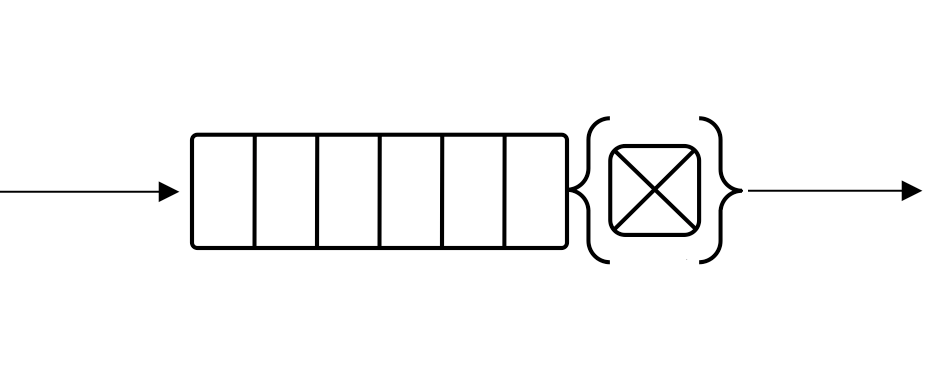
\includegraphics[width=\textwidth]{Images/MM12.png}
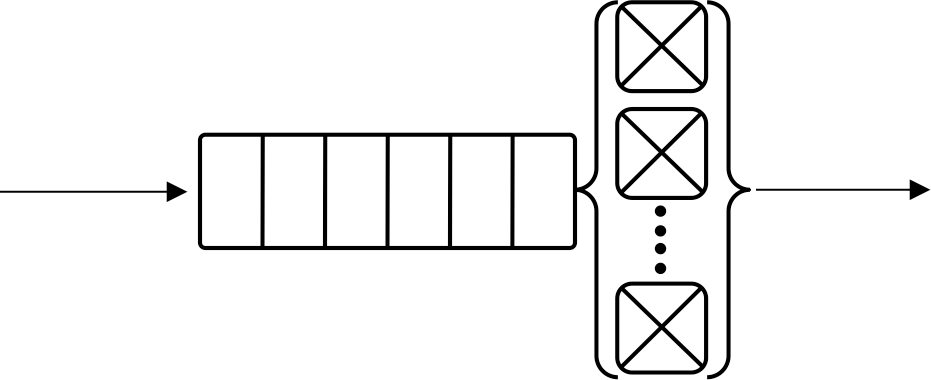
\includegraphics[width=\textwidth]{Images/MMc.png}
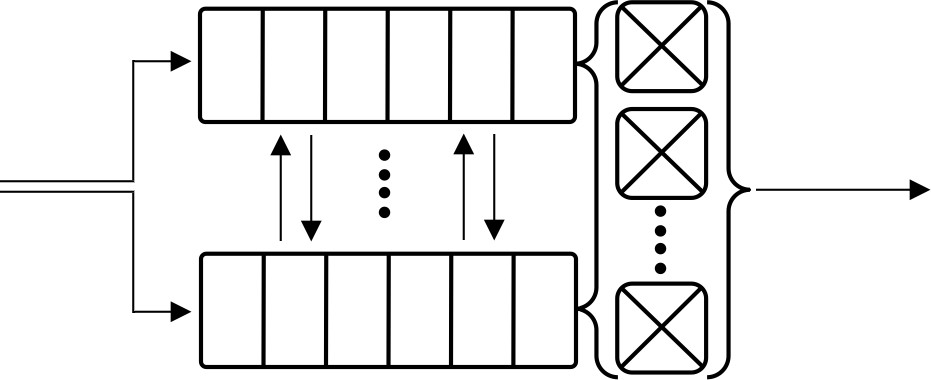
\includegraphics[width=\textwidth]{Images/Tandem.png}
\caption{\small Schematics of various queueing systems ($M/M/1$, $M/M/s/$, tandem); customers arrive from the left, enter the queue and progress through it until they are served, at which point the exit the queue.}\label{fig:MM}\hrule
\end{figure}\afterpage{\FloatBarrier}
\section{The $M/M/c$ Queuing System}
An $M/M/c/\textrm{GD}/\infty$ queueing system also has exponential inter-arrival and service times, with rates $\lambda$ and $\mu$, respectively. What sets this system apart is that there are now $c$ servers willing to serve from a single line of customers, perhaps like one would find in a bank (see Figure~\ref{fig:MM}). \par If $j \leq c$ customers are present in the system, then every customer is being served and there is no wait time; if $j > c$ customers are in the system, then $c$ customers are being served and the remaining $j - c$ customers are waiting in the line. \newl
To model this as a birth-death process, we have to observe that the death rate is dependent on how many servers are actually being used. \newpage\noindent If each server completes service at a rate of $\mu$ (which may not be the case in practice as there might be variations in servers... at least for human servers), then the \textbf{actual death rate} is $\mu \times$ the number of customers actually being served. The parameters for this process are
\begin{align*}
\lambda_{n} &= \lambda, \ n=0,1,2,\ldots \\ 
\mu_n &= n\mu, \ n=0,1,2, \ldots, c \\
\mu_{n} &= c\mu,\  n=c+1,c+2,\ldots 
\end{align*}
The traffic intensity for the $M/M/c$ system is $\rho = \lambda/(c \mu)$ and the steady-state solution is 
\begin{equation} 
 \pi_{n} = 
\begin{cases}
     \frac{\left(c \rho\right)^{n}}{n!} \pi_{0}      & \text{, $1\leq n \leq c$}  \\ 
     \frac{c^{c} \rho^{n}}{c!} \pi_{0}   & \text{, $n \geq c$} 
\end{cases}
\nonumber\qquad  \text{where  }
\pi_{0} = \left[1 + \frac{\left(c \rho\right)^{c}}{c! \left(1-\rho\right)} + \sum^{c-1}_{n=1} \frac{c \rho^{n}}{n!}\right]^{-1}.
\end{equation}
\normalsize  
Note that, as was the case in a $M/M/1$ system, if $\rho \geq 1$, there can be no steady state -- in other words, if the arrival rate is at least as large as the maximum possible service rate $\lambda \geq c \mu$, then the system ``blows up''.\newl From the client's point of view, there might be a desire to ensure that customers do not wait in line an inordinate amount of time, but there might also be a desire to minimise the amount of time for which at least one of the server is idle. In a $M/M/c$ queueing system, this steady-state probability is given by 
$$ P( n \geq c) =  \frac{\left(c \rho\right)^{c}}{c! \left(1-\rho\right)} \pi_{0}.$$ 
Table~\ref{tab:pns} shows $P( n \geq c)$ for a variety of situations depending on $s$ and $\rho$.  
\begin{table}[!t]
\centering
\begin{tabular}{ccccccc}
\hline
$\rho$ & $c=2$ & $c=3$ & $c=4$ & $c=5$ & $c=6$ & $c=7$ \\
 \hline
.10& .02& .00& .00& .00& .00& .00 \\
.20& .07& .02& .00& .00& .00& .00 \\
.30& .14& .07& .04& .02& .01& .00 \\
.40& .23& .14& .09& .06& .04& .03 \\
.50& .33& .24& .17& .13& .10& .08 \\
.55& .39& .29& .23& .18& .14& .11 \\
.60& .45& .35& .29& .24& .20& .17 \\
.65& .51& .42& .35& .30& .26& .21 \\
.70& .57& .51& .43& .38& .34& .30 \\
.75& .64& .57& .51& .46& .42& .39 \\
.80& .71& .65& .60& .55& .52& .49 \\
.85& .78& .73& .69& .65& .62& .60 \\
.90& .85& .83& .79& .76& .74& .72 \\
.95& .92& .91& .89& .88& .87& .85 \\
\hline
\end{tabular}
\caption[\small Probabilities that all servers are busy in an $M/M/c$ system]{\small Probabilities $P(n\geq c)$ that all servers are busy in an $M/M/c$ system for $c=2,\ldots, 7$ and values of $\rho$ between 0.1 and 0.95. \cite[p.1088]{QS_W}.}\label{tab:pns}\hrule
\end{table}\afterpage{\FloatBarrier}
Cumbersome calculations, using $W_{s} = \frac{1}{\mu}$, yield $$ L_{q} = P( n \geq c) \frac{\rho}{1-\rho}, \quad 
W_{q} = \frac{L_{q}}{\lambda}, \quad
W = \frac{1}{\mu} + W_{q}, \quad\mbox{and}\quad
 L = \frac{\lambda}{\mu} + L_{q}.$$
\newpage\noindent Consider, for instance, a bank with two tellers. An average of 80 customers arrive at the bank each hour and wait in a single line for an idle teller. For this specific bank, the average service is 1.2 minutes. Assume that inter-arrival times and service times are exponential. Determine:
\begin{itemize}[noitemsep]
	\item[(a)] The expected number of customers in the bank.
	\item[(b)] The expected length of time a customer spends in the bank.
	\item[(c)] The fraction of time that a particular teller is idle.
\end{itemize}
We are dealing with an $M/M/2$ system with $\lambda =80 $ customers/hr and $\mu = 50$ customers/hr. Thus, $\rho = \frac{80}{2\cdot 50} = 0.80 < 1$ and the steady-state exists. 
\begin{itemize}[noitemsep]
	\item[(a)]  From the above table, $P(n \geq 2) = 0.71$, from which we compute 
\begin{align*} L_{q} &= P( n \geq 2)\cdot \frac{.8}{1-.8} = 2.84 \text{ customers}\\
L& = 	\frac{80}{50} + L_{q}	= 4.44 \text{ customers.} \end{align*}
\item[(b)]	We know that $W = \frac{L}{\lambda} = \frac{4.44}{80} = 0.055 \text{ hr }= 3.3 $ min.
\item[(c)] To determine the fraction of time that a particular server is idle, note that tellers are idle during all moments when $n=0 $, and half the time (by symmetry) when $n = 1$. The probability that a server is idle is thus given by $ \pi_{0} + 0.5 \pi_{1}$. But
 $$\pi_{0} = \left[1 + \frac{\left(2\cdot .8\right)^{2}}{2! \left(1-.8\right)} + \sum^{2-1}_{n=1} \frac{2\cdot .8^{n}}{n!}\right]^{-1}= \frac{1}{9} \quad\mbox{and}\quad \pi_{1} = \frac{1.6}{1!} \pi_{0} = 0.176$$ and so the probability that particular teller is idle is $0.11 + 0.5(0.176) = 0.198$.
\end{itemize}
\textbf{IMPORTANT NOTE:} other queueing models are not understood to the same extent, and their given performance measurements may only be approximate and highly-dependent on the specifics of the problem at hand. For this reason, $M/M/c$ models are sometimes used even when their use is not supported by the data (the situation is not unlike the wide use of the normal distribution). In various applications, the empirical distributions of arrivals and service times are nearly Poisson and exponential, respectively, so that the assumption is not entirely missing the mark, but numerical simulations should not be eschewed when departures from the $M/M/c$ model are too pronounced.
\section{Application: Wait Time at Canadian Airports}
By providing efficient and effective \textbf{pre-board screening} (PBS), the \textit{Canadian Air Transport Security Authority} (CATSA) ensures the safety of all passengers and crew aboard flights departing Canadian airports while maintaining an appropriate balance between staffing and the wait time experienced by passengers. \par The number of active screening stations and the number of passengers affect the wait times, and, as a result, budget cuts have a strong impact on the system, both in Canada and in the United States.\newpage\noindent
Numerous factors influence the wait time at pre-board screening checkpoints at Canadian airports: the schedule intensity of departing flights, the volume of passengers on these flights, the number of servers and processing rates at a given checkpoint, etc. \par One of CATSA's goals is to ensure that the pre-board screening experience at Canadian airports is made as efficient as possible by minimizing the waiting time at checkpoints. With this in mind, the \textbf{Wait-Time Impact Model} (WTIM) was designed to achieve the following tasks: 
\begin{enumerate}[noitemsep]
\item provide estimates of the passenger arrival rates $\lambda$, the processing rates $\mu$ and the number of servers $c$ at each checkpoints, using available field data;
\item calculate the Quality of Service (QoS) level $(p_x,x)$  and determine what service level can be achieved at each checkpoint (i.e. the percentage $p$ of passengers which will wait less than $x$ minutes, for $x$ fixed) for a given arrival rate $\lambda$, processing rate $\mu$, number of servers $c$;
\item provide the average number of servers $c^*$ required to achieve a prescribed QoS level $(p_x,x)$, given an arrival profile $\lambda^*$;
\item provide quality of service (QoS) level curves $(p_x (x),x)$ (i.e. cumulative distribution curves) under various arrival rate and number of active servers for each checkpoint (where $x$ is allowed to vary).\end{enumerate}
The \begin{figure}[!t]
\centering
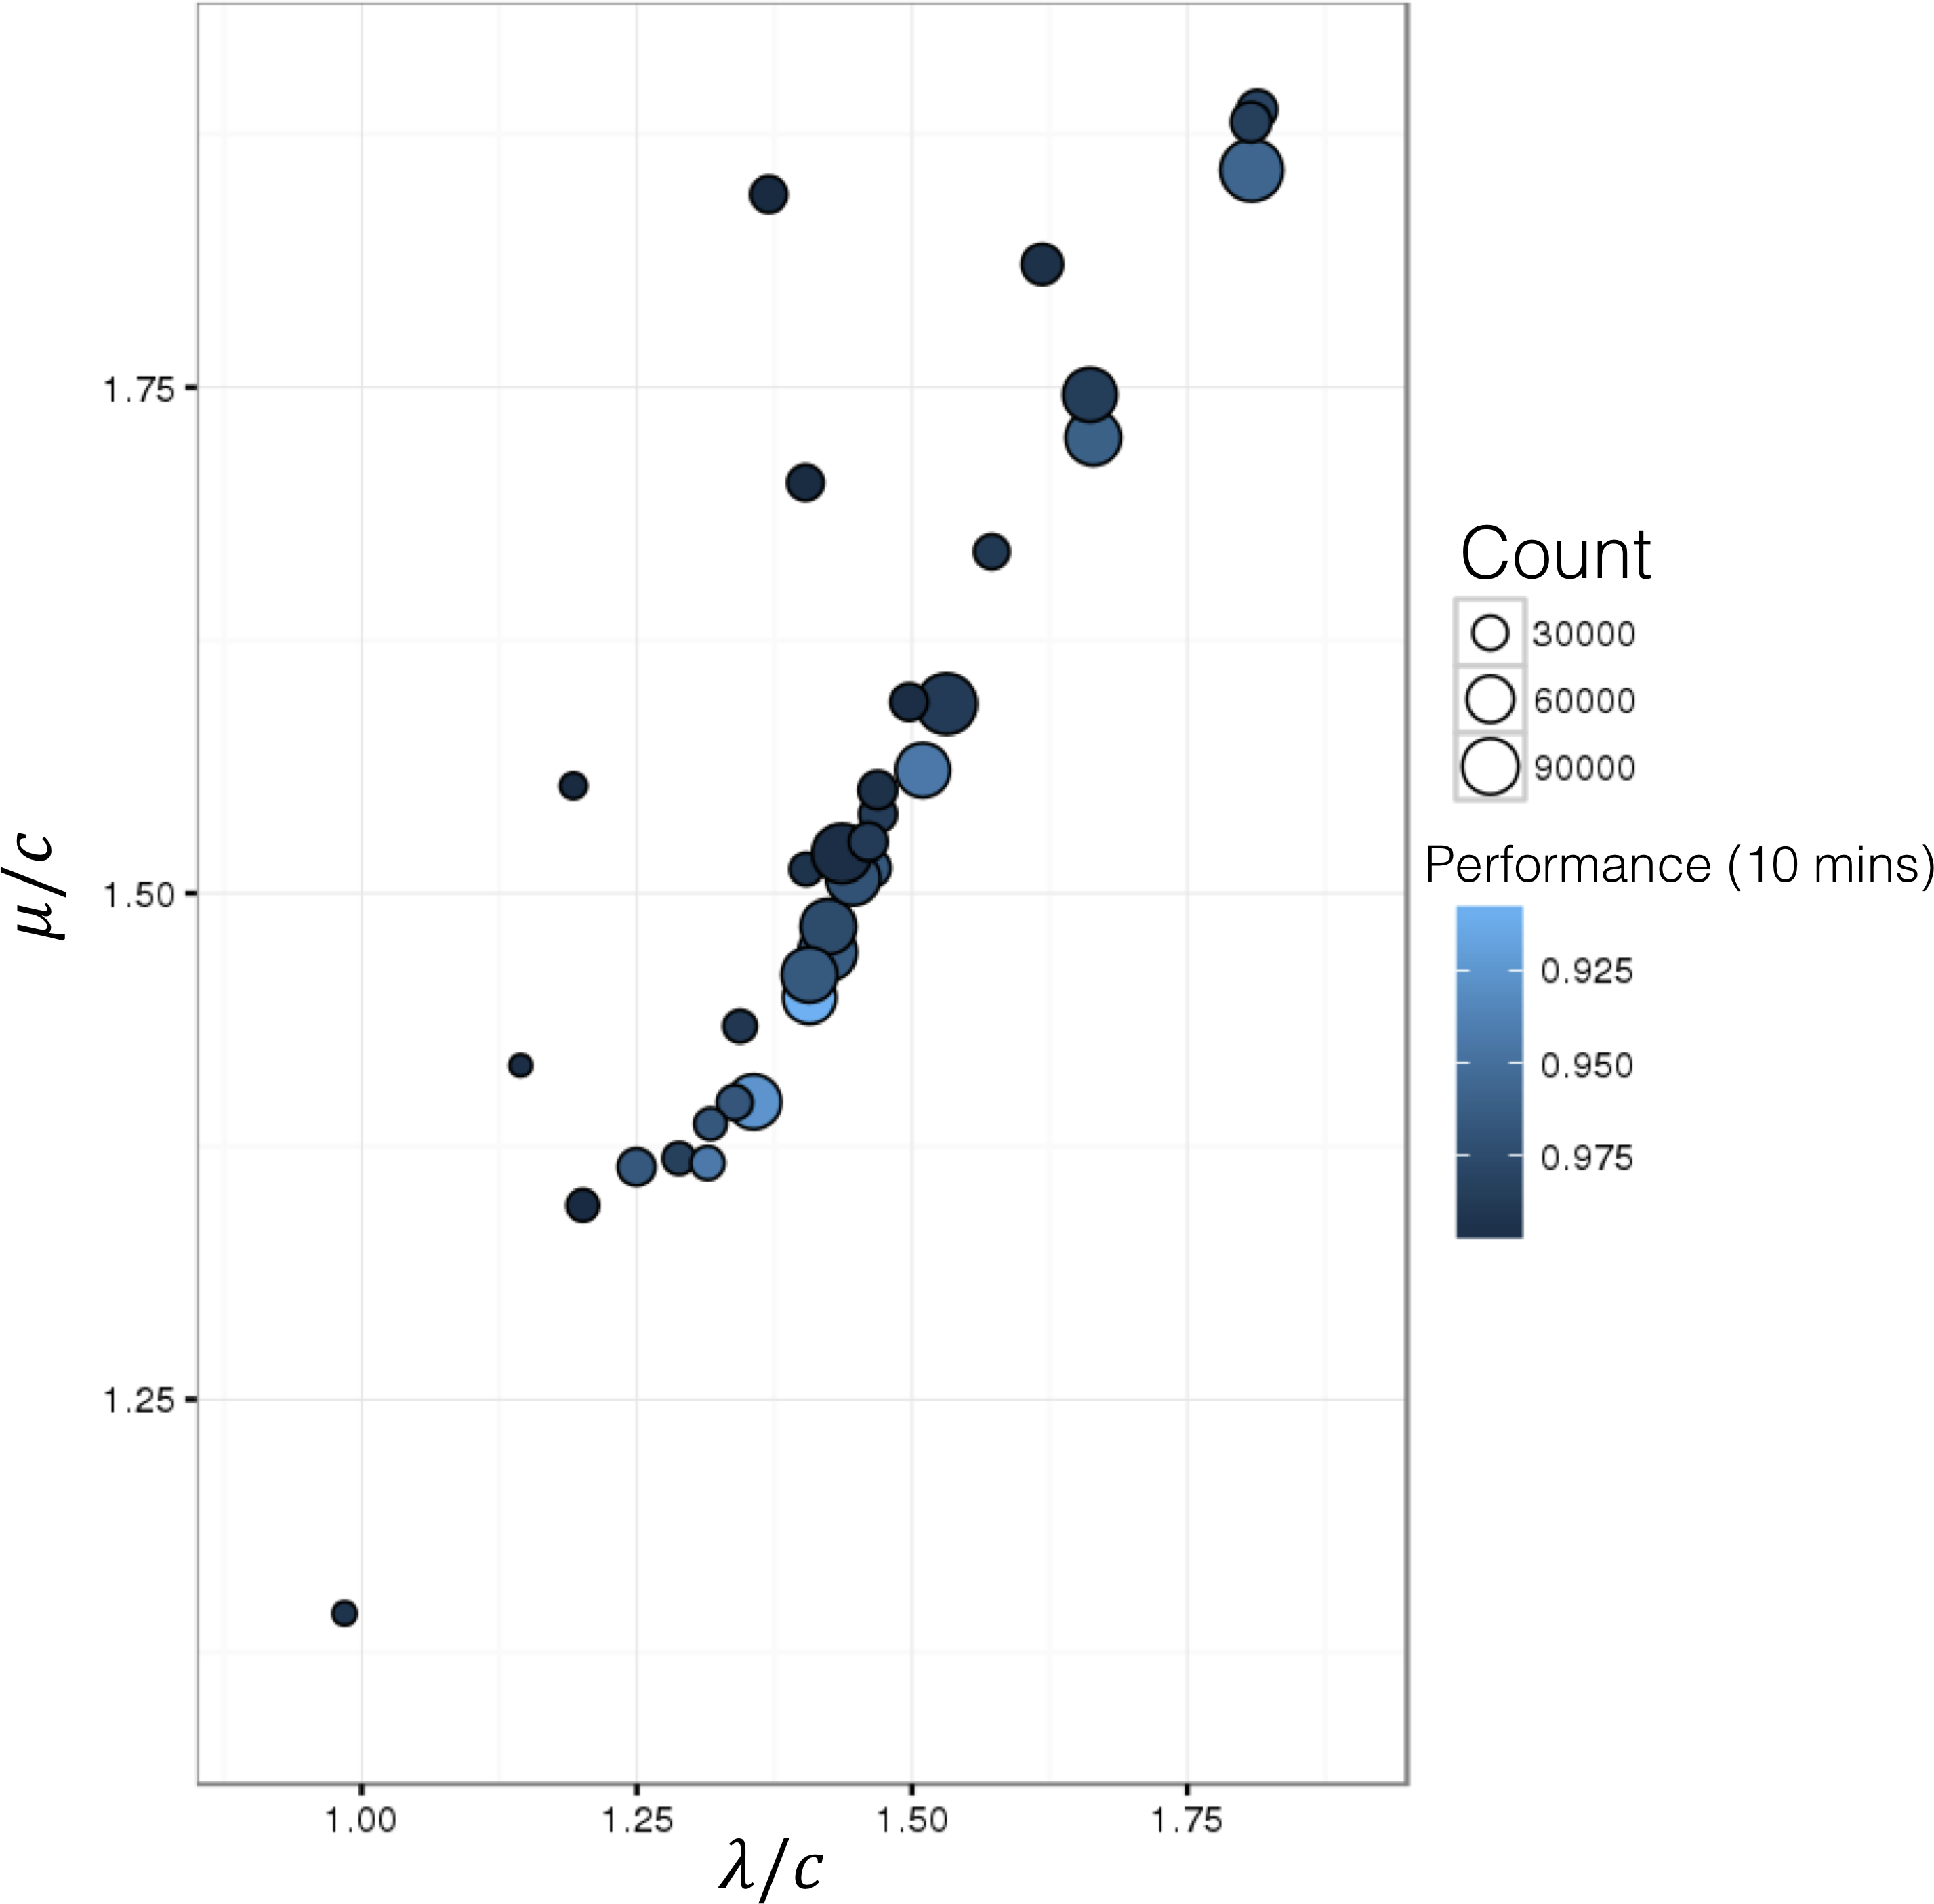
\includegraphics[height=0.42\textheight]{Images/CATSA2.png}\quad 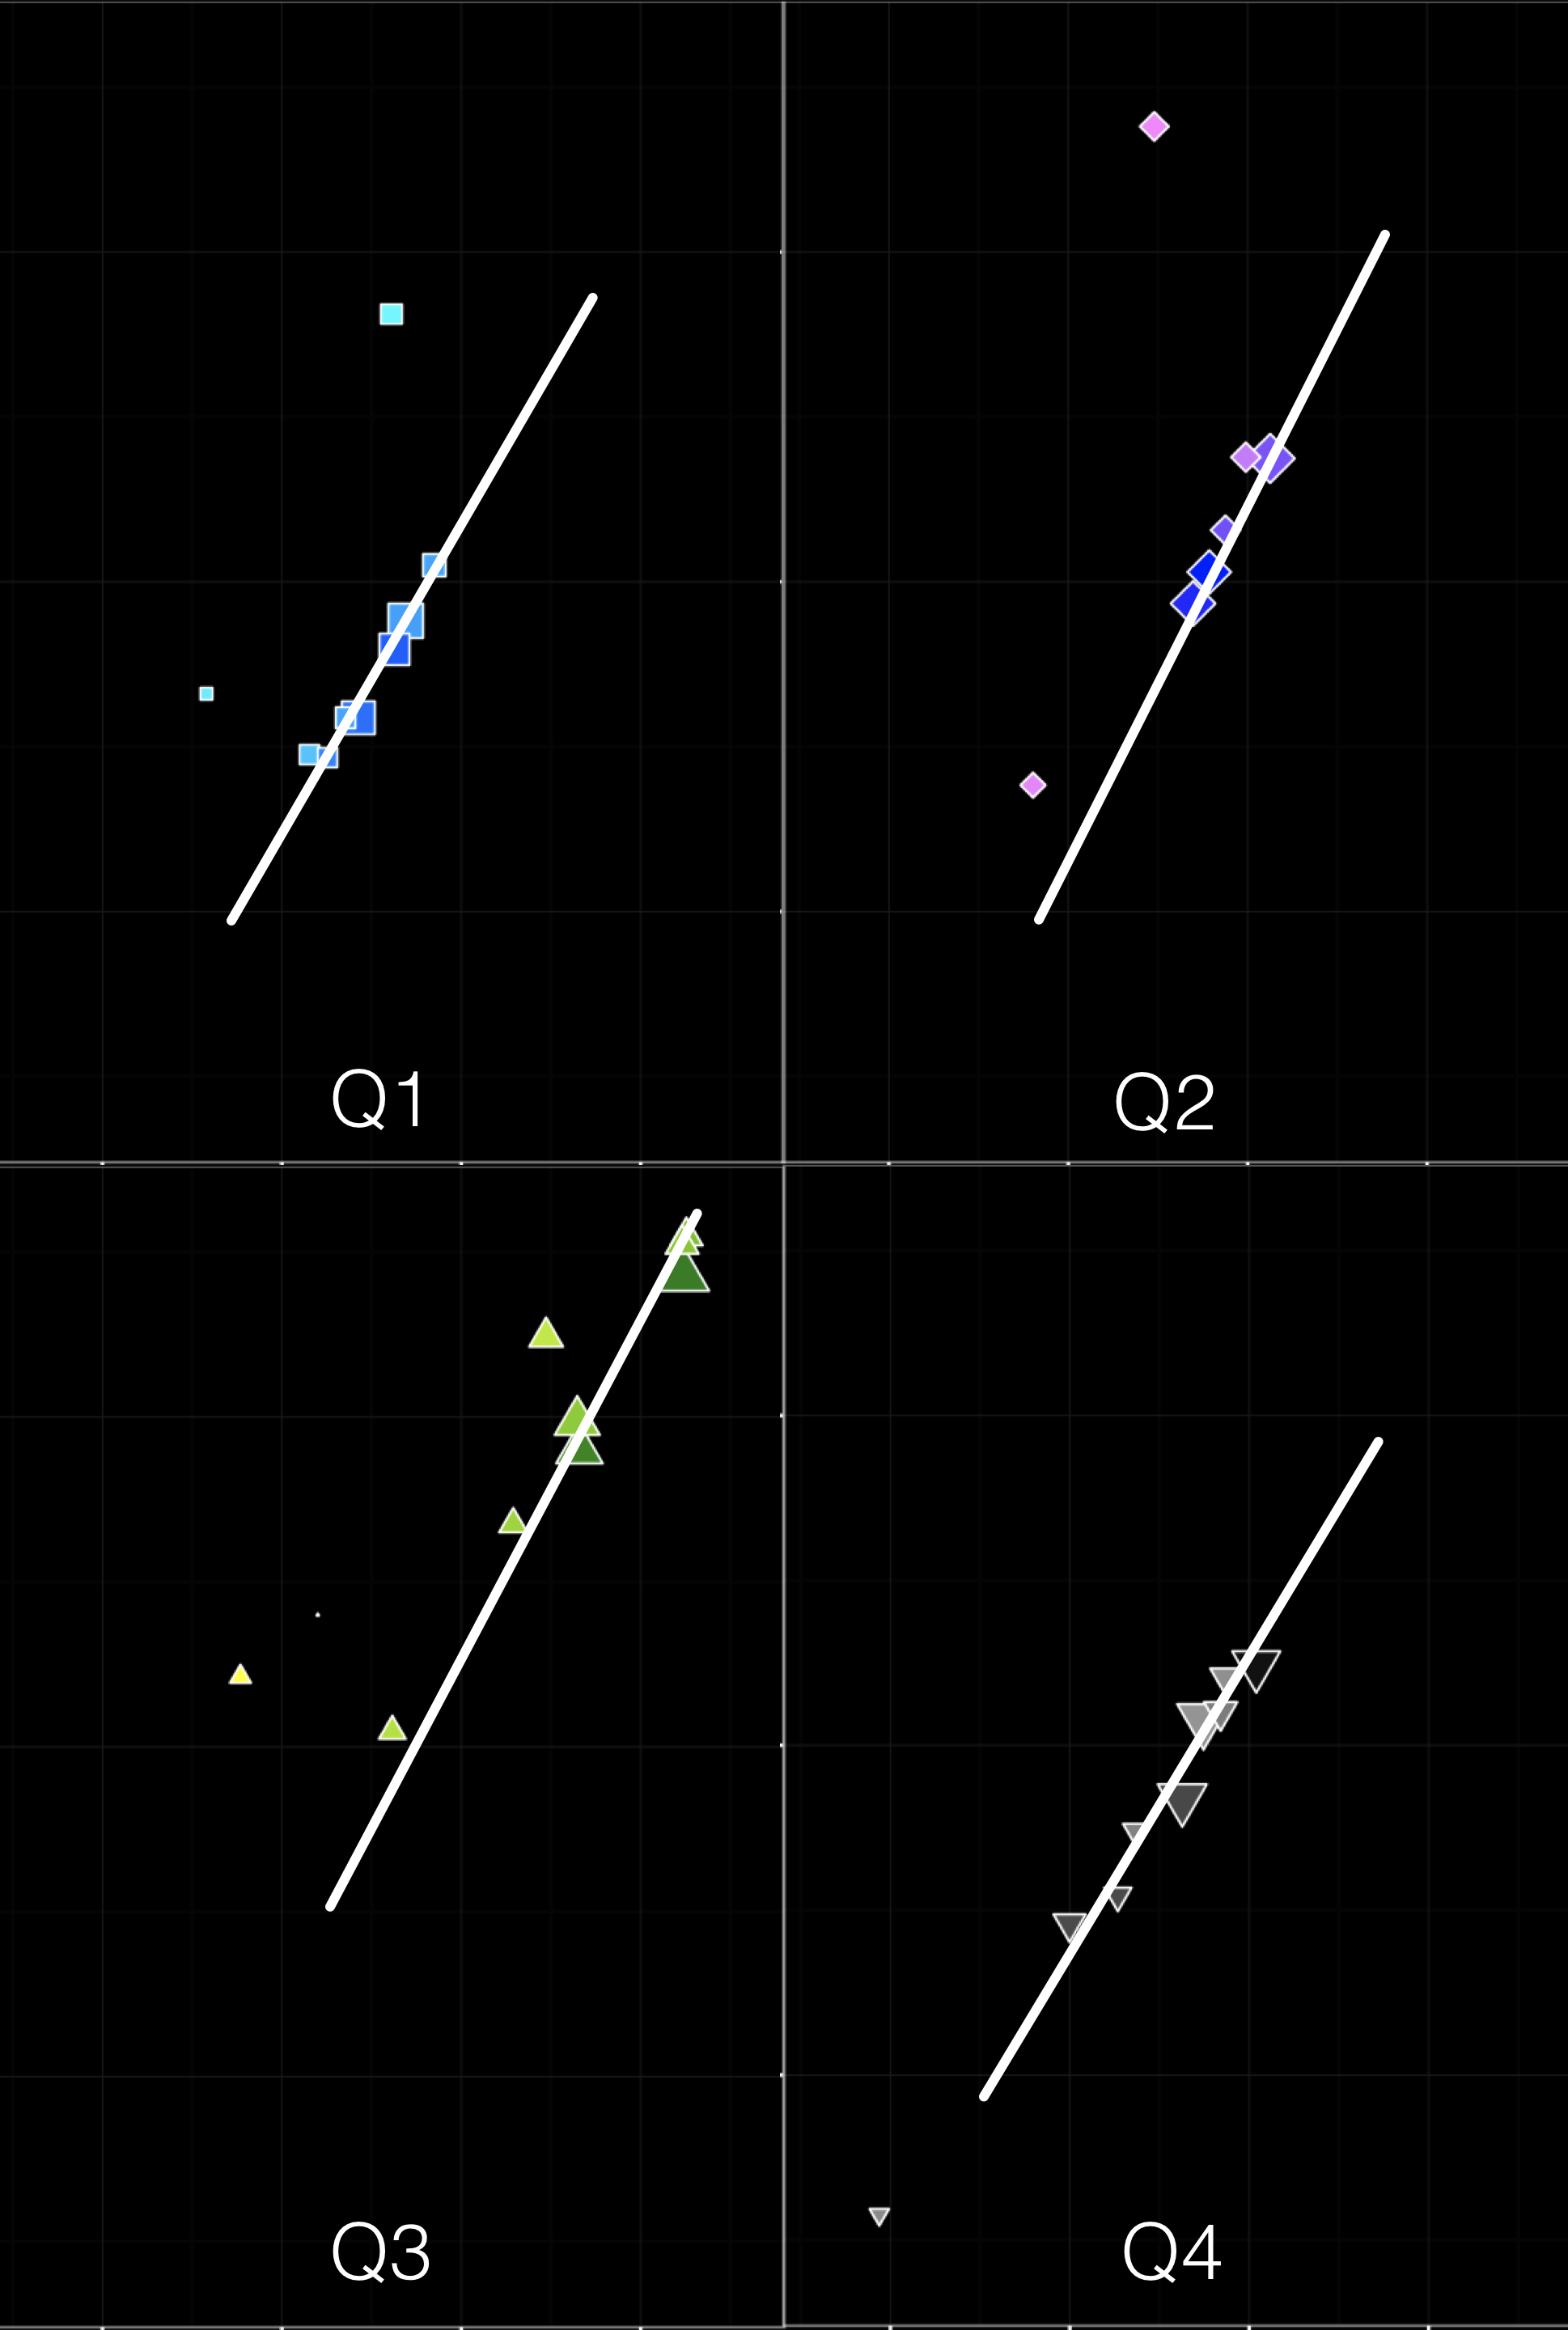
\includegraphics[height=0.42\textheight]{Images/CATSA3.png}  
\caption[\small Visualisation of a checkpoint's queueing parameters]{\small Visualisation of a specific checkpoint's queueing parameters -- $\lambda$, $\mu$, $\bar{c}$, passenger count, and performance (percentage of travellers waiting less than 15 minutes to be screened); the relationship between $\lambda/\bar{c}$ and $\mu/\bar{c}$ is practically linear (left), which is easier to see at the quarter level (right).}\label{fig:checkpoint}\hrule
\end{figure}\afterpage{\FloatBarrier}
 queueing structure leads to some interesting insights  (see Figure~\ref{fig:checkpoint}). The prediction's quality are seen in Figure~\ref{fig:predsCATSA}. Details are available in the Project Summary, as well as in the Final Report (extract). 
\newpage\noindent
\begin{figure}[H]
\centering
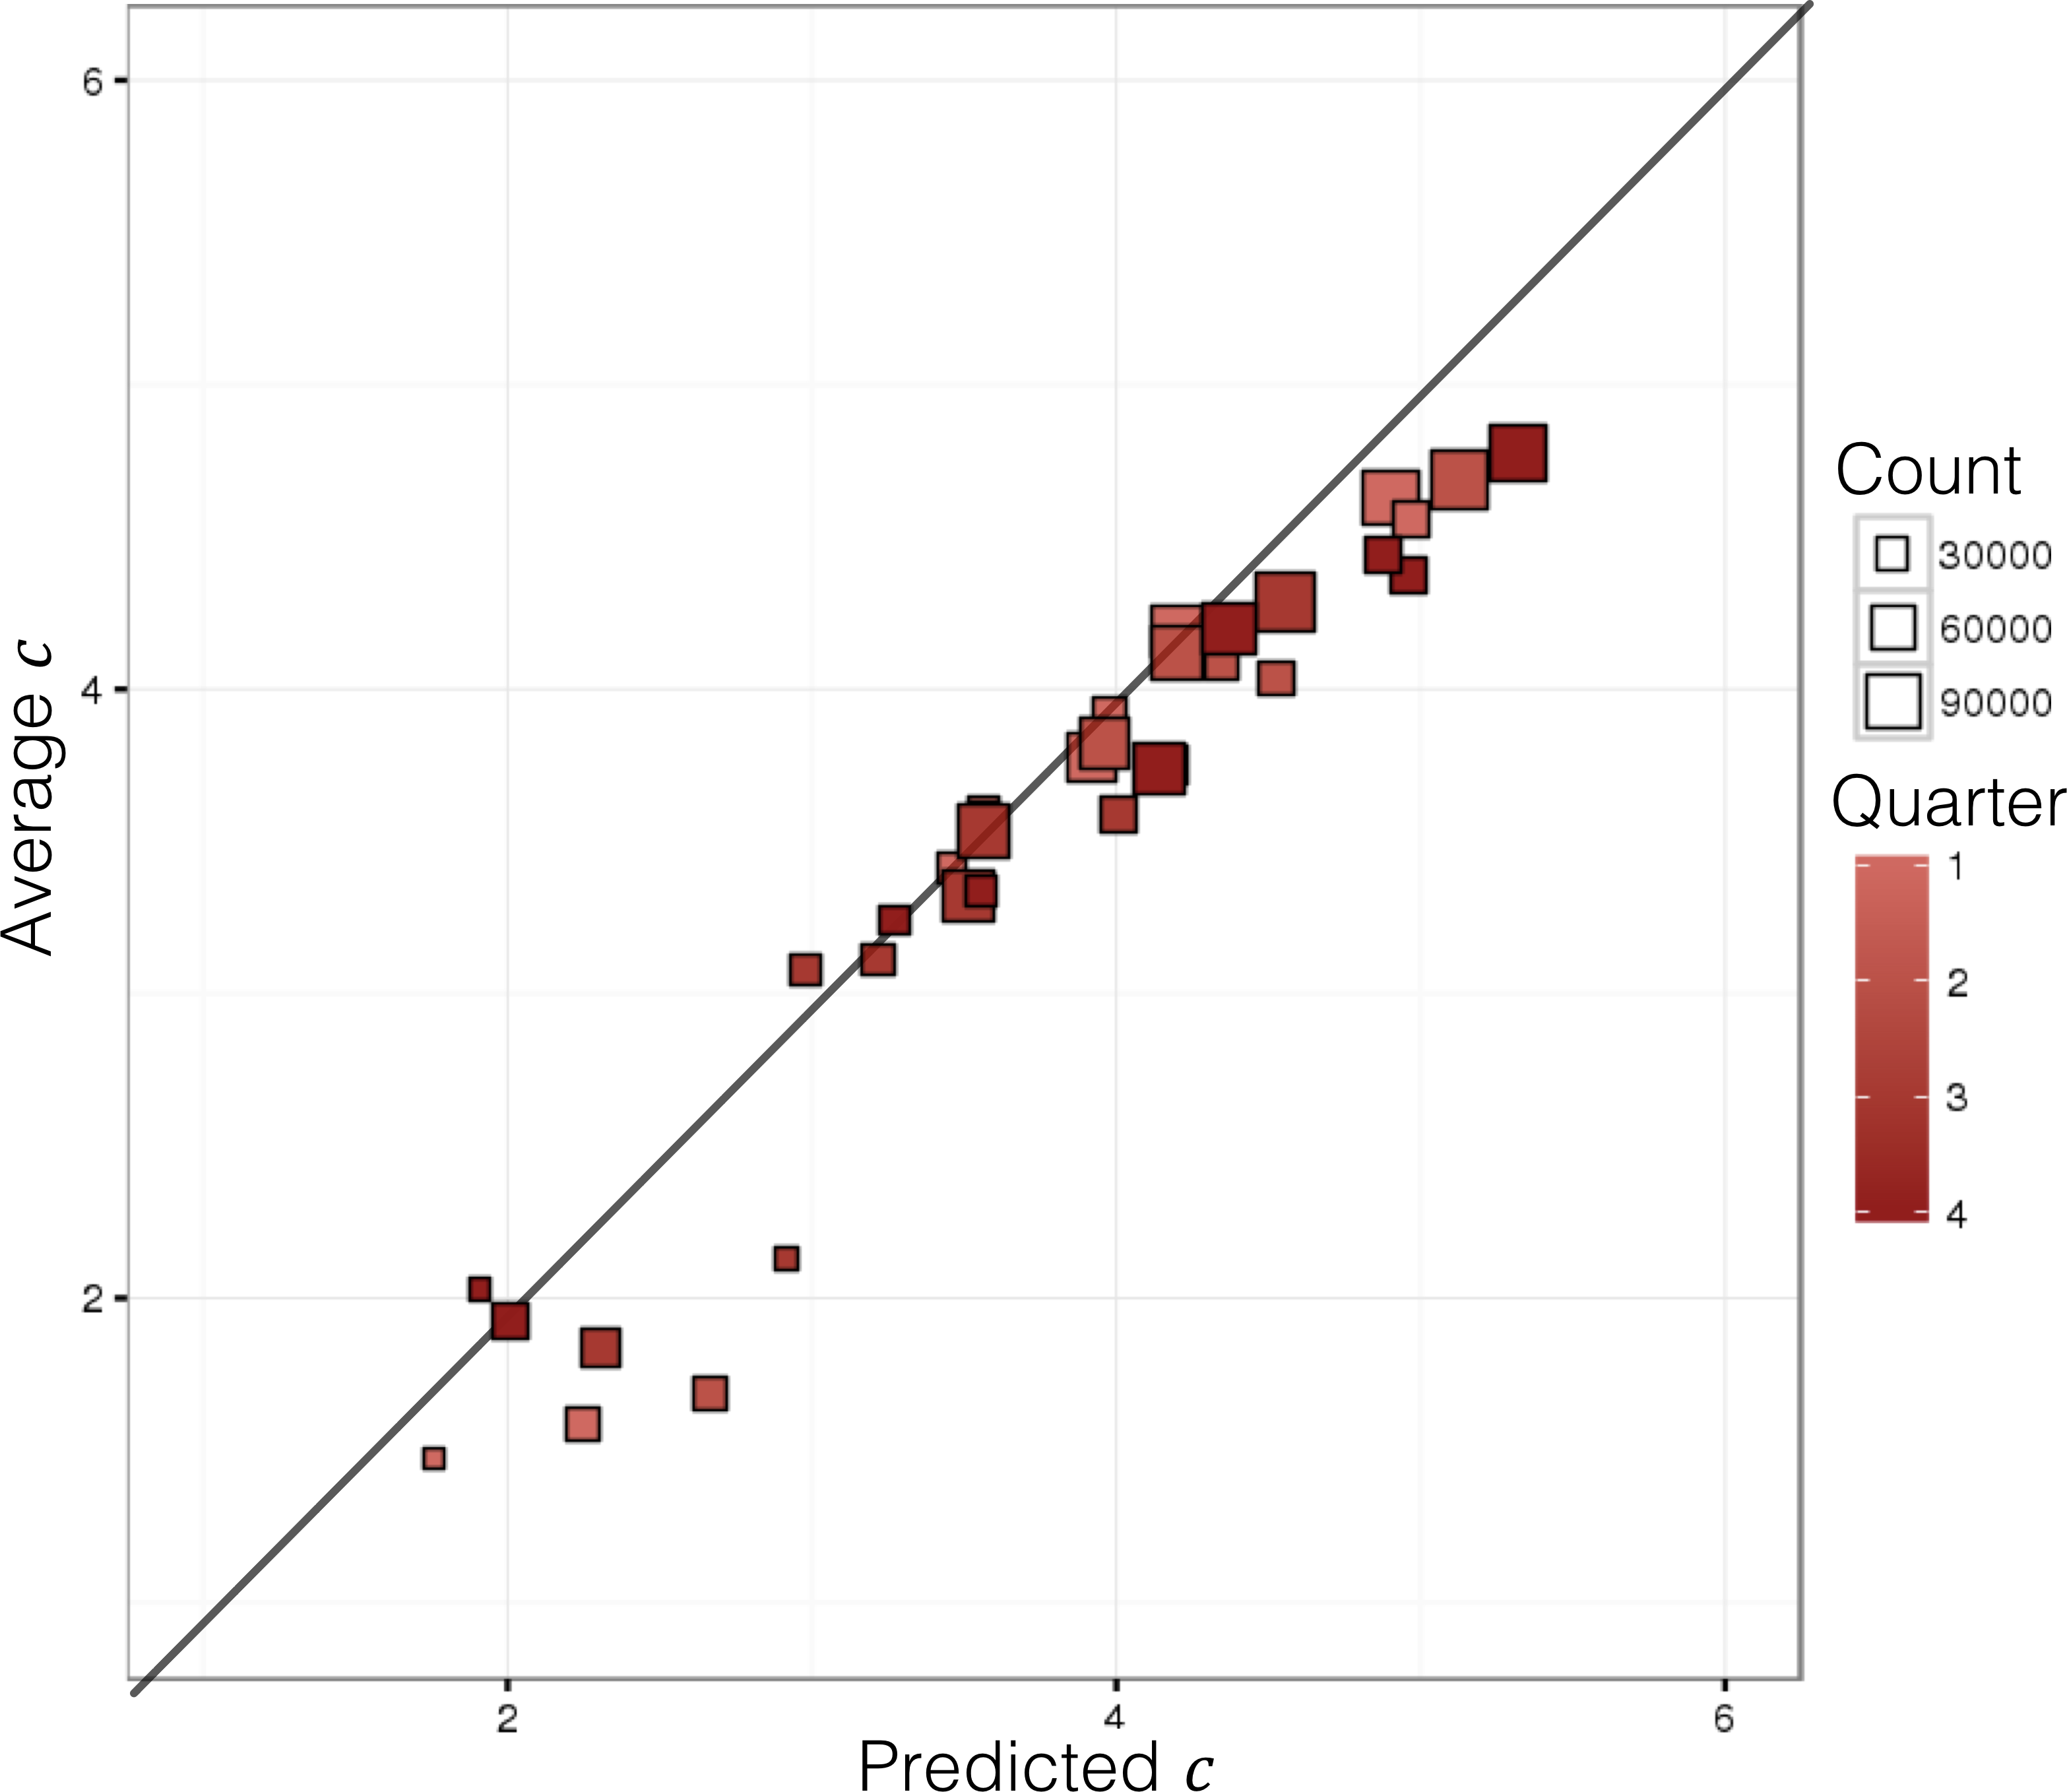
\includegraphics[width=0.55\textwidth]{Images/CATSA4.png}  
\caption[\small Predicted number of servers]{\small Predicted average number of server against actual number of server required to maintain prescribed performance, with passenger count, by quarter. The perfect prediction line is added for ease of comparison.}\label{fig:predsCATSA}\hrule
\end{figure}\afterpage{\FloatBarrier}
